\documentclass[a4paper]{report}

%\usepackage{ifpdf}
%\ifpdf 
%\usepackage[pdftex, pdfauthor={Yan King Yin}, bookmarks, anchorcolor=blue, colorlinks, linkcolor=blue, citecolor=blue, urlcolor=blue, breaklinks]{hyperref}
%\else 
%\usepackage[dvipdfm, pdfauthor={Yan King Yin}, bookmarks, anchorcolor=blue, colorlinks, linkcolor=blue, citecolor=blue, urlcolor=blue, breaklinks]{hyperref}
%\fi
\usepackage[dvips, pdfauthor={Yan King Yin}, bookmarks, anchorcolor=blue, colorlinks, linkcolor=blue, citecolor=blue, urlcolor=blue, breaklinks]{hyperref}
\usepackage{breakurl}
\usepackage[dvips,final]{graphicx}
\usepackage{float}
\usepackage[square]{natbib}
\usepackage{color}
\usepackage{pstricks}
% \usepackage{algorithmic}
% \usepackage{algorithm}
\usepackage{amsmath}   % for {equation} {cases}
\usepackage{amssymb}   % for \curlyvee
\usepackage{stmaryrd}  % for \bigcurlyvee, \widetilde{\bigwedge}
\usepackage{wasysym}   % for \iint (double integral)
\usepackage{makeidx}
\usepackage[style=list,acronym=true,number=none]{glossary}
\usepackage{alg}
\usepackage{minitoc}
\usepackage[pointedenum]{paralist}
\usepackage[sf,bf,big,raggedright,compact]{titlesec}
%\usepackage{pslatex}

\renewcommand{\familydefault}{\sfdefault} 
\renewcommand{\mtcfont}{\small\sffamily}
\renewcommand{\mtcSfont}{\small\sffamily}
\renewcommand{\mtcSSfont}{\small\sffamily}
\renewcommand{\mtcSSSfont}{\small\sffamily}
\renewcommand{\mtifont}{\small\sffamily}
\renewcommand{\mtctitle}{}
\renewcommand{\chaptername}{Ch }

\titlespacing{\chapter}{0pt}{0pt}{0pt}
\titleformat{\chapter}[hang]{\sffamily\bfseries\Huge}{\thechapter \hspace{30pt}}{0pt}{}

%\renewcommand{\algorithmicrequire}{\textbf{Input:}}
%\renewcommand{\algorithmicensure}{\textbf{Output:}}
%\renewcommand{\algorithmiccomment}[1]{// \textit{#1}}
\newcommand{\algrepeatforever}{\textbf{repeat forever}\\\algbegin}

\interfootnotelinepenalty=50000

\title{\textbf{Genifer\\-- an artificial general intelligence}}
\author{Yan King Yin (general.intelligence@Gmail.com)\\ \\
with input from:\\
Abram Demski\\
Ben Goertzel\\
Martin Magnusson\\
Russell Wallace\\
Pei Wang
}
\date{\copyright May 2009 -- version 0.8}

\setlength{\headheight}{0cm}
\setlength{\hoffset}{0cm}
\setlength{\topmargin}{-2cm}
\setlength{\oddsidemargin}{-2cm}
\setlength{\evensidemargin}{-2cm}
\setlength{\textwidth}{19cm}
\setlength{\textheight}{28.5cm}
\setlength{\headsep}{0cm}
\setlength{\topskip}{0cm}
\setlength{\footskip}{0.5cm}  % between bottom of page and page number
\setlength{\floatsep}{0cm}
\setlength{\textfloatsep}{0.6cm}
\setlength{\intextsep}{0.5cm}
\setlength{\parindent}{0em}
\setlength{\parskip}{7pt}
\setlength{\pltopsep}{-5pt}   % for compact-enum
%\setlength{\partopsep}{5pt}
%\setlength{\plparsep}{5pt}
\pagestyle{plain}

\includeonly{logic}
% \includeonly{business-aspects}
\makeindex
\makeglossary

\begin{document}
\maketitle
%\setcounter{chapter}{-1}
\dominitoc
\tableofcontents

\chapter{Introduction}
\begin{flushright}
\emph{I am an enthusiast, but not a crank in the sense that I have some pet theories as to the proper construction of a flying machine. I wish to avail myself of all that is already known and then, if possible, add my mite to help on the future worker who will attain final success.}\\
--- Wilbur Wright
\end{flushright}

\begin{flushright}
\emph{Everything should be made as simple as possible, but no simpler.}\\
--- Albert Einstein (rephrased)
\end{flushright}

\begin{flushright}
\emph{An inventor is simply a fellow who doesn't take his education too seriously.}\\
--- Charles Kettering 
\end{flushright}

\begin{flushright}
\emph{When a subject becomes totally obsolete we make it a required course.}\\
--- Peter Drucker
\end{flushright}
%\begin{flushright}
%\emph{A problem well stated is a problem half-solved.}\\
%--- Charles Kettering
%\end{flushright}
\minitoc

This book describes a theory of AGI (Artificial General Intelligence) \citep*{Goertzel2007} that is still being developed.  I think the AGI problem can be decomposed into $\sim$10 computational issues and we will somehow integrate them together:

\leftskip 1cm
knowledge representation\\
fuzzy-probabilistic logic\\
deduction\\
abductive reasoning\\
inductive learning\\
pattern recognition / categorization\\
belief revision\\
memory organization\\
natural language\\
sensory processing

\leftskip 0cm
My approach is predominantly symbolic / logic-based, but it also employs redundancy in knowledge representation, and in this sense is somewhat like neural networks.  Also, it may merge with neural networks at the sensory level.  This approach can be called ``neo-classical AI''.

I try to make this book as easy to understand as possible.  Also, the theory remains open to new ideas and suggestions.

This book focuses on theoretical aspects of AGI.  The source code of $\mbox{Genifer}$ is hosted on \href{http://launchpad.net/genifer}{LaunchPad} and this \href{http://www.geocities.com/genericAI}{older website} contains additional information not transferred to this book yet.  Also feel free to \href{mailto:Generic.Intelligence@Gmail.com}{contact me}!

\section{Some background of AI}

The word ``logic'' comes from \textit{logos} which can mean ``word'', ``thought'', or ``reason''.  The study of logic is the study of the \textbf{mechanisms of thinking}.  Aristotle (ca 350BC) is often credited with the first substantial study of logic, with a focus on syllogisms.  Our current system of logics was developed by people such as De Morgan (1840s), Boole (1840s), Frege (1879, \textit{Begriffsschrift}), Russell and Whitehead (1903, \textit{Principia Mathematica}), and others (including Liebniz (1670s, ``algebra of thought'') whose work remain undiscovered till the 1880s).

\textbf{Logic-based AI}\\
Thus it is not so surprising that the design of AI can be based on logic.  John McCarthy (who coined the term ``AI'' in a 1956 Darthmouth conference) was first to propose the use of \textbf{formal logic} in AI.  Herbrand (1908-1931) created a basis of provability in predicate logic.  In 1965, Robinson discovered the \textbf{resolution} method for logical inference, which enabled the creation of \textbf{logic programming} and the language Prolog (Kowalski and Colmerauer, 1970s).

\textbf{Connectionism}\\
In 1943, McCulloch and Pitts formulated a formal model of neurons, leading to Rosenblatt's Perceptron (1957), and later the computational paradigm of artificial neural networks (ANNs).  In the 1980s there was a resurgence of interests in ANNs and connectionism due to the invention of the backpropagation algorithm for multilayer perceptrons.  At this point it was recognized that connectionism has the strengths of \textbf{robustness} and \textbf{graded response}, in contrast to logic-based AI's \textbf{brittleness} and \textbf{bivalence}.

\textbf{Recent trends}
In the 1990s there was rapid development in \textbf{statistical learning}.  It was then realized that ANN learning algorithms are a special case of statistical learning.  Recent development in AI is distanced from ``GOFAI'' (Good Old-Fashioned AI) by their use of statistical learning, \textbf{sub-symbolic representations}, and \textbf{optimization methods} (computational intelligence).  Computational intelligence includes new paradigms such as evolutionary computing (drawing inspiration from sexual reproduction) and swarm intelligence (drawing from social interactions).

\section{Why logic?}
\label{sec:why-logic}

I started designing AGI using the neural network approach for a few years, until I discovered some fundamental difficulties in the NN approach, so I switched to a more logic-based one\footnote{Though my approach is not purely logic-based.}.

Logic-based AI went out of vogue beginning in the 1980s because of the advent of connectionism and later statistical learning methods.  As a result, many researchers nowadays are unfamiliar with even the basics of logic-based AI.  In order to understand my approach it is extremely important to be familiar with \textbf{first-order logic} (FOL) and to understand the difference between first-order representations and propositional ones.

\textbf{Propositional vs first-order.}  This is a typical propositional statement:\\
\hspace*{1cm} $ p \vee q \wedge r $\\
and a typical first-order statement:\\
\hspace*{1cm} $ p(X) \vee q(X,Y) \wedge r(w(Y,Z)) $\\
The chief distinction is the use of \emph{variables} in first-order logic, which greatly increases its expressiveness.

The vast majority of statistical learning literature assumes that the data is represented by points in a high-dimensional space.  I call this the ``spatial'' approach which includes methods like nearest neighbor, support vector machines (SVMs), principal component analysis (PCA), and artificial neural networks (ANNs).  \textit{Spatial datasets are equivalent to propositional representations.}  First-order logic is a symbolic or relational\footnote{Relational representations are a subclass of first-order representations that do not allow functors and structured terms.} approach which is qualitatively very different.  There is strong evidence that some datasets can be easily learned by relational methods but are very difficult, if not impossible, to learn with spatial methods.  (\citep*{Thornton1996}, \citep*{Thornton2000}.\footnote{He demonstrated this with the example of a ``checkerboard'' pattern of 0's and 1's that can be easily learned by a logical formula, but would be very difficult for a neural-network learner.  This is actually the age-old debate between symbolic AI and connectionism, given a new twist in the context of machine learning.} provides an interesting and detailed analysis of this issue.)

To put it more bluntly, I suspect that propositional approaches are rather useless in the logic-based AI framework (but I'd be pleasantly surprised to learn otherwise).

Notice in the figure below, that all \textbf{spatial classifiers} work by ``chopping'' the space of data points (shown in 2D here) into various regions with the use of hyper-planes (as a line in 2D) or some curved boundaries.  This is very different from how first-order logic classifies data.

\begin{figure}[H]
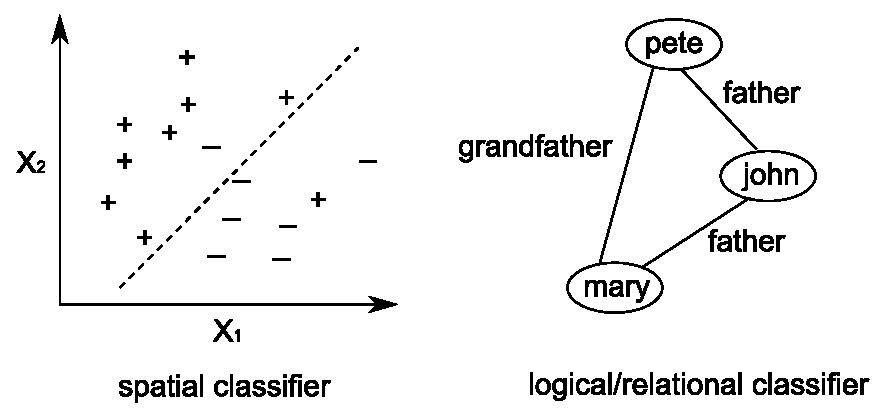
\includegraphics{spatial-vs-logical.eps}
\caption{Spatial vs logical classification}
\end{figure}

To illustrate this with an example:  Let's think of how a child (AGI or human) learns the concept of (blood) relatives.  The child (Jane) would be given some examples of people around her and whether they are her relatives, eg:\\
\hspace*{1cm} father(jane, john), relative(john)\\
\hspace*{1cm} mother(jane, mary), relative(mary)\\
\hspace*{1cm} uncle(jane, pete), relative(pete)\\
\hspace*{1cm} neighbor(jane, joe), $\neg$relative(joe)\\
\hspace*{1cm} friend(jane, kate), $\neg$relative(kate)\\
and the task is to learn a general rule for relatives.  The solution can be stated quite succinctly\footnote{This solution is not entirely correct, as relatedness can grow unbounded and everyone would be ultimately blood-related.  Perhaps this problem can be resolved by fuzziness and other mechanisms such as non-monotonicity, but my point here is to show that the situation for propositional representation is even worse, as the problem appears insurmountable in that case.} in first-order logic:\\
\hspace*{1cm} relative(X, Y) $\leftarrow$ parent(X, Y)\\
\hspace*{1cm} relative(X, Y) $\leftarrow$ sibling(X, Y)\\
\hspace*{1cm} relative(X, Y) $\leftarrow$ married(X, Y)\\
\hspace*{1cm} relative(X, Y) $\leftarrow$ relative(X,Z), relative(Y,Z)\\
but it is very difficult to express in propositional logic unless we limit the domain of entities to a few people.  Also, we can see that \textit{spatial} statistical learning will fail to learn this rule because:\\
1. The dataset cannot be represented as numerical values in a vector space, or it could be done only very awkwardly.\\
2. Even when the dataset is cast in vector space, the learning algorithm can mostly learn to classify \textit{existing} examples, but the \textit{generalizations} would be wrong -- this is because the formulae in first order logic can entail discrete examples that are not necessarily located in a localized region in the numerical space.  Even if you carve the space into ridiculously complex regions, the next example would still be an exception because ``spatial compactness'' is simply absent in the underlying concept.\\
3. The child's world typically has very few people in it, yet she is able to learn the concept.  In ANNs and statistical learning, the sample size is typically at least 100s, but logic-based learning can learn the concept with just a few examples.

Although first-order representations can be converted to propositional ones via the process of propositionalization, such algorithms cost exponential time and space.  This is not difficult to see:  FOL allows us to express knowledge very succinctly.  There are some techniques that ameliorate the combinatorial explosion, such as partial instantiation (\citep*{Chandru1999}) or sparse matrix (\citep*{Domingos2008}).  But I still think it is easier and more intuitive to working on a FOL KB directly, especially for AGI.

And, despite propositionalization, the class of spatial statistical learning techniques still seem to be unsuitable for logic-based AGI because propositionalization does not cure the fundamental lack of ``spatial compactness'' in logical structures that I pointed out above.  (After propositionalization, some fast propositional SATisfiability algorithms can be invoked, but they are still qualitatively different from the spatial learning algorithms.)  As a result of this, my current strategy is to focus on algorithms specifically for FOL.

\{ Update:  \citep*{Gartner2008} describes a general method to construct kernels for (first-order and higher-order) logic formulae, based on a representation of logic by typed lambda calculus formulated by \citep*{Lloyd2003}.  This may be a bridge between logical and spatial methods, but I have not looked into it in detail.  Also, the theory of topoi and categories may offer a way to construct morphisms between models of logic theory and geometric spaces (cf Joseph Goguen's unified concept theory and theory of institutions).  Also, \citep*{Muggleton2005} developed a support-vector ILP method. \}

\{ Some new techniques have been developed to lift neural networks to first-order representations, but I have not examined them in detail (eg, \citep*{Garcez2009}).  \}

\section{Why not neural network?}

There are several reasons why I think the NN approach may be less promising:

1.  First-order logic is a more powerful representation scheme than (feed-forward) neural networks (\S\ref{sec:why-logic}), whereas dynamic neural networks are very difficult to work with.

2.  A neuron is "fixed" within a network and cannot "move around", which seems to make it difficult to perform invariant pattern recognition (eg, translational, rotational, and scale- invariance in vision). The brain has to use neurons due to biological constraints, but it seems more effective to use other pattern matching methods on von Neumann machines. (Scale invariance is particularly difficult for ANNs, see \citep*{Muresan2004}.)

3.  Neural learning is slower and require a larger amount of examples. Logic-based learning is coarse-grained and thus require fewer examples to induce the correct representation, sometimes as few as 1 example.

4.  As Ben Goertzel pointed out some years ago, a network of redundant propositions can be reduced to a minimum number of non-redundant propositions, without loss of information;  the only thing that is lost is \textit{fault tolerance}.

However, neural networks may be used for handling low-level vision, especially at the feature-extraction level.

\section{Recursive self-improvement}
\label{sec:RSI}

RSI refers to the ability of an AGI to reprogram itself.  Some authors predict that the RSI point will trigger the Technological Singularity (eg \citep*{Kurzweil}).  I think the way to reach the RSI point with the least amount of efforts would be to build an automatic program synthesis tool that accepts natural-language commands or goal specifications.  From then on, we can use this tool to rewrite the tool itself and to evolve it (semi-automatically) into a full AGI system.

\section{Chicken-and-egg problem}
\label{sec:chicken-and-egg}

\begin{figure}[H]
\centering
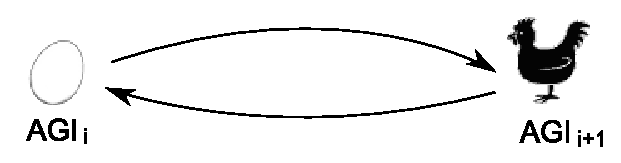
\includegraphics{chicken-and-egg1.eps}
%\caption{chicken and egg problem}
\end{figure}
\vspace{-0.5cm}

Anyone who has thought about AGI long enough will be aware of this problem:  The idea is to use a ``program evolver'' that takes an input program $\Pi_i$ and improves it to $\Pi_{i+1}$ according to some user-specifications.  We put the evolver through itself, thus building up its intelligence recursively without doing any programming (except for the initial evolver).

This idea (at least naively) does not work because the initial evolver needs to have very good background knowledge about programming or else it cannot perform its job in reasonable time.  \S\ref{sec:self-programming-architecture} discusses how to make it feasible.

\section{Natural reasoning}
\label{sec:natural-reasoning}

Other names for natural reasoning are: common-sense reasoning, human-like reasoning, informal reasoning.

Natural reasoning is an extension of logical reasoning with:\\
1.  ability to recognize natural concepts (which I posit requires fuzzy pattern recognition)\\
2.  ability to use metaphors, similes, analogies, and similarity-based reasoning

An example of natural reasoning is:

\leftskip 1cm \textit{Suppose I need to write a program to ``break English sentences into words''.  I'd need to declare a function to do this.  What would be the input and output of this function?}

\leftskip 0cm Note that in the above reasoning, I think of the function as a ``box'' with something that goes in and something out.

Natural reasoning is required to turn informal, natural-language statements into formal statements.  This is especially important to formal program synthesis.

\chapter{Architecture}
\minitoc

We will first look at various basic architectures and then try to decide on a final design.

\section{Logic-based blackboard architecture}

This is an older design I explored around 2006, chiefly to put together several logic-based algorithms on a blackboard.  The following page is a schematic diagram showing various modules of the \textbf{logical sub-system}.

My intuition is that such a logical sub-system is essential to any AGI, but it should be built on top of a more basic, \textit{procedural} layer (cf \S\ref{sec:proc-subsumes-decl}, ``Procedural subsumes Declarative'').

\begin{figure}[H]
\centering
\includegraphics[width=5.65625in,height=2.9895833in,bb=0 0 543 287]{CompleteArchitecture2-small.png}
%\caption{AGI architecture}
\end{figure}

\section{BDI architecture}

BDI (\textbf{belief-desire-intention}) is one of the most successful agent architectures ever proposed.  It was first investigated by Michael Bratman as a theory of human practical reasoning (\citep*{Bratman1987}), and later formulated as an agent architecture (\citep*{Bratman1988}).  The main concern of BDI is how to plan in the face of a \textit{dynamic environment} and with \textit{bounded resources}.

Key to BDI is the idea of \textbf{commitment}.  Once an agent commits to a plan, the plan will constrain means-end reasoning, thus making planning processes more efficient.

\textbf{B: Beliefs} are the contents of the KB.\\
\textbf{D: Desires} are unconstrained;  they need not be achievable or even consistent (eg, one can desire smoking and good health at the same time).\\
\textbf{I: Intentions} are goals that the agent commits to;  they are believed to be achievable and must be consistent.

\begin{figure}[t]
\centering
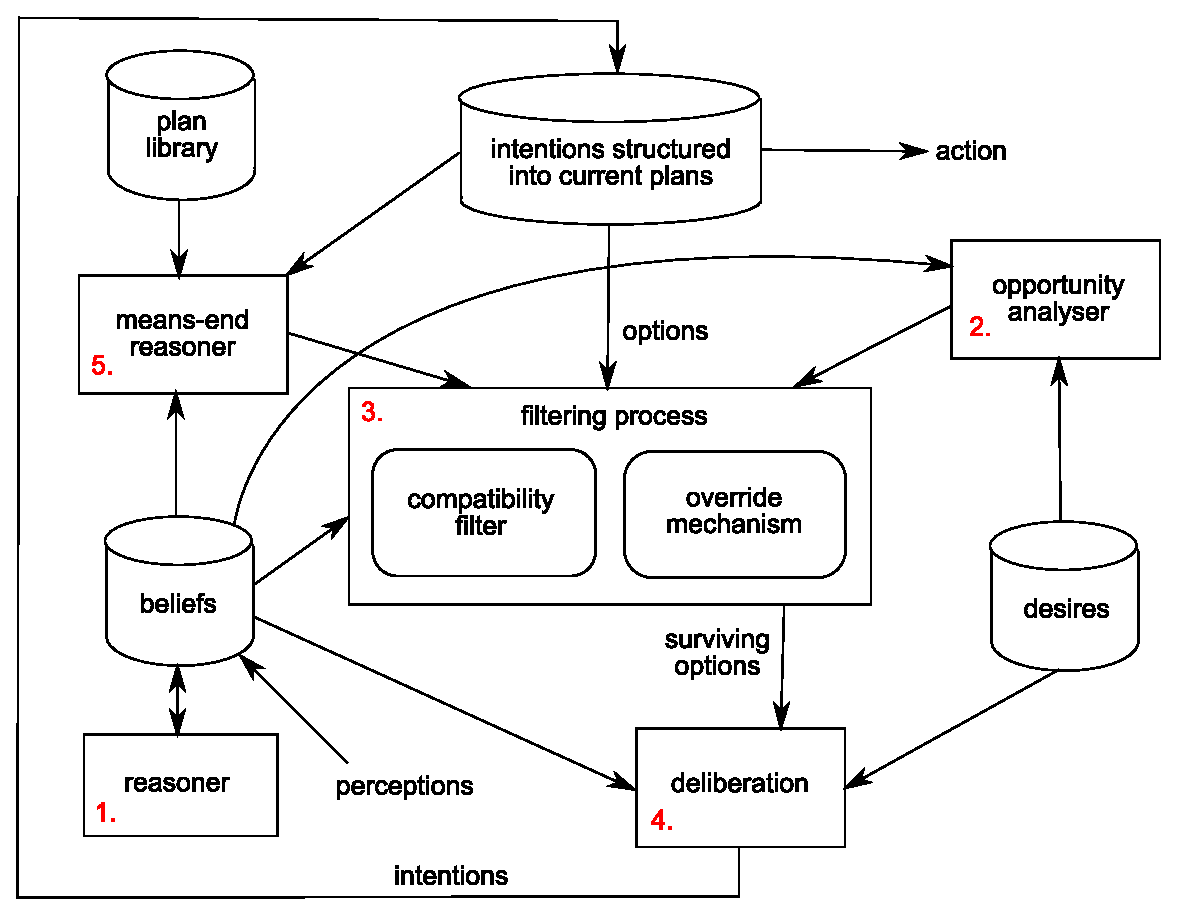
\includegraphics[scale=0.6]{BDI-architecture.eps}
\caption{schematic diagram of the BDI architecture}
\label{fig:BDI-arch}
\end{figure}

Figure \ref{fig:BDI-arch} is a schematic diagram of BDI.  The key processing steps are:
\begin{compactenum}
\item  This is the \textbf{Knowledge / Declarative Sub-system}, which we will consider at length in the rest of the book.
\item  Changes in the environment cause changes in beliefs, which in turn reveal new possibilities to satisfy desires.  Thus the \textbf{Opportunity Analyzer} tries to propose new \textbf{options}.
\item  Once the options are produced (either by the Opportunity Analyzer or the Means-end Reasoner), they are subject to \textbf{filtering}.  The \textbf{Compatibility Filter} checks if options are compatible with existing plans.
\item  Surviving options are weighted against each other by the \textbf{Deliberation Process}, which produces intentions to be incorporated as plans.
\item  The \textbf{Means-end Reasoner} searches for the next available options, taking into consideration the current plans.
\end{compactenum}

\section{Hayek architecture}

Hayek is an artificial economy proposed by Eric Baum (\citep*{Baum2004}) as an AGI architecture.  A slight variant of Hayek can be described as follows:

\begin{compactenum}
\item The AGI is composed of a large number of small programs.
\item \textbf{Cooperativity}.  The programs may call each other.
\item \textbf{Persistent memories}.  Individual programs can remember things across time slices.
\item A \textbf{meta-controller} runs these programs according to some schedule, allotting each program a time slice.
\item \textbf{Credit assignment}:  If the program answers a question correctly or performs a good action (judged by some external critic), the meta-controller will credit the programs that have contributed to the result.
\item Human programmers may contribute to this pool of programs.\\
\end{compactenum}

A high-level programming language (such as Lisp) seems to be more suitable for this purpose.

Note that even very complex algorithms can be implemented in this architecture.  For example, a best-first search algorithm can remember its search state in an external memory store.  Then it just waits for its time-slice to resume searching.  Thus human programmers can seed the artificial economy with highly competent programs.

\section{Decision-theoretic architecture}

This is mathematically more elegant than the BDI architecture.

Some important elements that should be present in the architecture:\\
1.  \textbf{percepts} are raw (unprocessed) sensory events\\
2.  \textbf{beliefs} are the contents of the KB\\
3.  \textbf{states} --- all possible \textit{perceived} states of the environment, including the current state.  States are special terms in the logic.\\
4.  \textbf{actions}\\
5.  \textbf{utility function} --- a function $U: \{states\} \rightarrow \mathbb{R}$.  Utilities may be defined implicitly, though.

This architecture may depend on a \textbf{logical sub-system} that:\\
1.  recognizes environmental states (eg \textit{``the apple is on the table''}) from raw percepts (eg pixel values from a camera)\\
2.  recognizes possible actions (eg \textit{``I can put the apple on the plate''})

The goal is to maximize expected utility.  Planning becomes a discrete optimization problem in this setting.

It seems that reinforcement learning \index{reinforcement learning} can be included in this architecture.

\section{Self-programming architecture}
\label{sec:self-programming-architecture}

Consider this variant of the chicken-and-egg problem (\S\ref{sec:chicken-and-egg}), where we distinguish between the \textbf{Synthesizer} and the AGI:
\begin{figure}[H]
\centering
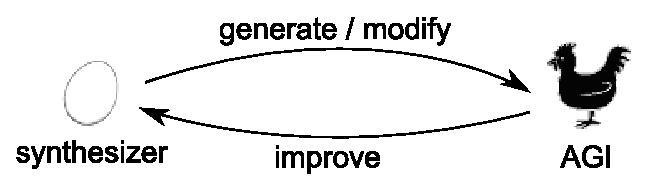
\includegraphics{self-programming-architecture.eps}
%\caption{improved self-programming architecture}
\vspace{-0.5cm}
\end{figure}

Currently we know the following program-synthesis paradigms:\\
1.  human programming\\
2.  natural reasoning (NR), ie common-sense / human-like reasoning\\
3.  automated theorem proving (ATP)\\
4.  stochastic local search (SLS), including evolutionary algorithms (EA)\\
5.  reinforcement learning (RL) \index{reinforcement learning}\\
We will consider each paradigm in turn.

A key question is how an initially-dumb AGI can \textit{improve} the performance of the Synthesizer, even slightly.

\textbf{1. Human programming} (ie, brute-force software engineering without RSI)\\
The problem with this approach is that it does not exploit the advantages of machine program synthesis, and thus is likely to be sub-optimal.

\textbf{2. Natural reasoning} (cf \S\ref{sec:natural-reasoning})
\begin{compactenum}[(a)]
\item  The problem is that NR does not yet exist, but it is a \textit{sine-qua-non desideratum} of AGI.
\item  So the question is how to enable an initially weak form of NR to synthesize programs.  One possibility is to use \textbf{creativity}:  the AGI will generate programs by partly reasoning and partly random acting.
\item  An agent with NR is likely to have RL as well.
\item  An NR agent can invoke ATP.
\item  An NR agent can self-program (without invoking ATP), simply by \textbf{deductive planning} (\S\ref{sec:deductive-planning}).\\
\end{compactenum}

\textbf{3. ATP}
\begin{compactenum}[(a)]
\item  It requires \textit{formal} specifications of programs (or sub-routines), which are often very hard to write for humans.
\item  Search in proof space can be very slow.
\item  There already exists ATP-based program synthesis software, which can be used externally.\\
\end{compactenum}

\textbf{4. Stochastic local search}
\begin{compactenum}[(a)]
\item  Is based on generate-and-test.
\item  ``Generate'' is random and the program space is typically huge.
\item  ``Test'' is often slow because it requires the entire AGI to answer a large number of benchmark queries.  A possible remedy is to specify input-out benchmarks for AGI \textit{components}, but then the burden is on humans to design the modular architecture.
\item  A large population of relatively low-score programs has to be maintained, in order to allow sufficient time for cooperativity to evolve.  For this reason I suspect that the evolutionary approach is rather slow.
\item  2 further problems are:  How can an initially-dumb AGI improve the stochastic searcher?\footnote{In MOSES (cite) an attempt is made at ``representation building''.} And how can this transfer of rationality from the AGI to the Synthesizer be coded once and for all?\\
\end{compactenum}

\textbf{5. Reinforcement learning} \index{reinforcement learning}
\begin{compactenum}[(a)]
\item  The goal of RL is to learn policies of how to act in certain environmental states.  It can synthesize programs if the environment is that of programming.
\item  RL can be augmented with logical reasoning.\\
\end{compactenum}

\textbf{Combining all methods}\\
Apparently, we can combine all the above methodologies without conflict:
\begin{figure}[H]
\centering
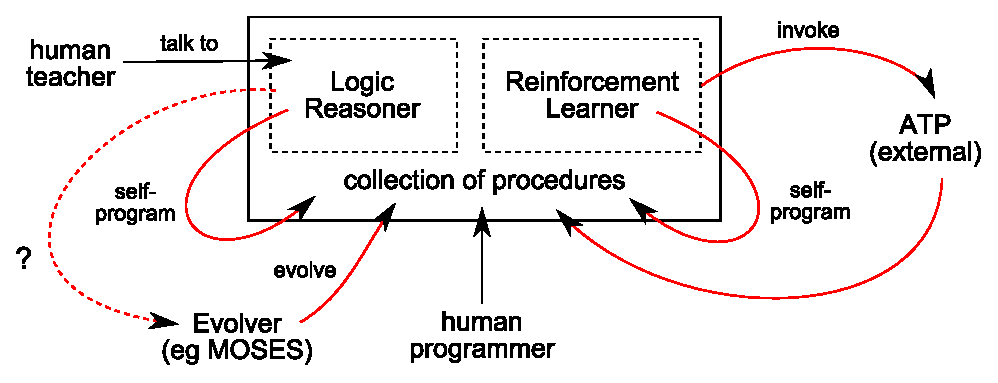
\includegraphics{combined-architecture.eps}
\vspace{-0.5cm}
\end{figure}

The question is to choose the \textit{most effective} method of AGI self-programming (red lines).  My intuition is that the evolutionary method is much less efficient than the other 3 (it is easier to explain to children to do something than to train animals by reinforcement, which is in turn easier than breeding animals for the innate ability to do that thing), provided that some rudimentary ability of reasoning is present.

Maybe the most cost-effective method (from the human labor perspective) is to combine RL with logical reasoning and deductive planning --- for instance, to allow RL to invoke logic or vice versa.

\{ TO-DO:  what about means-end reasoning?  utility maximization? \}

\chapter{Knowledge representation}
\minitoc

\section{Introduction}

What would be a good knowledge representation scheme for AGI?  We need to understand that there is no single right answer to this question.  An AGI uses a KR structure to \textit{represent} the external world, and this KR structure is built with limited computational resources.  As such, it must be an approximation of the world.  This means we have much freedom in the choice of KR.

My choice is based on classical logic, especially first-order logic (FOL) because of its well-established status in AI research.  Also, FOL is easy for myself and others to understand.

A common misconception is:  ``How can complex ideas such as `John loves Mary' be reduced to logic formulae like \textit{loves(john,mary)}?''  One school of thought (see eg \citep*{Johnson-Laird1983}) posits that human reasoning is based on ``mental models'', but it is unclear how exactly they can be constructed.  My view of logic-based AI is that of using logic (or ''relational formalisms'') as a \textit{computational structure} for \textit{constructing} mental models.  It does not mean that logical formulae in an AGI correspond to ``Truths'' in the real world.

TO-DO:  Typed or untyped logic?

\section{Reification}
\label{sec:reification}

TO-DO:  explain what is reification, how it is represented.

\section{Composition functor}
\label{sec:CompositionFunctor}

\section{Rus logical form}
\label{sec:Rus-logical-form}

\section{Representing time}

As Einstein would have said, the representation scheme for space and time should be fundamentally the same.  As I have developed a vision theory (\S\ref{ch:vision}), I think temporal representations can follow a similar scheme.  OpenCog (http://www.opencog.org) is an AGI project more focused on embodiment, so we can also share their KR scheme.

\section{Assumptions and counterfactuals}

How to make assumptions during inference?  ``Assuming mom is at home, I call her phone number''.

Example of a counterfactual conditional:  ``If Oswald did not kill JFK, someone else would have''.

\section{Contexts}

An excellent survey of contexts in logic-based AI is \citep*{Akman1996}.

\chapter{Logic}
%\begin{flushright}
%\end{flushright}
\minitoc

Note:  This chapter is currently very chaotic because of a re-organization effort.  $\mathcal{Z}$ is no longer considered a foundational part of the logic.

\section{Background}

\subsection{Turing completeness}

\textbf{Undecidability of FOL.}

\subsection{$\lambda$ calculus}

(See Wikipedia: \href{http://en.wikipedia.org/wiki/Lambda_calculus}{Lambda calculus}).

\textbf{Bound variables:}  In the abstraction $(\lambda x.t)$ we call $x$ the bound variable and $t$ the body.  Every occurrence of $x$ in $t$ is \textbf{bound} by the abstraction.  Conversely, an occurrence of a variable $y$ is \textbf{free} if it is not bound, eg in $(\lambda z.(\lambda x.(yx)))$.

\textbf{Head-normal form:}  A $\lambda$ term is in head-normal form if, for $m \geq 0$ and $n \geq 0$, it can be expressed as:
$$\lambda x_1 ... x_m . x t_1 ... t_n$$.
The variable $x$ may either be free or bound (one of $x_1,...,x_m$).

\textbf{De Bruijn indexes.}

\textbf{Director strings.}

\subsection{Combinatory logic}

(See Wikipedia: \href{http://en.wikipedia.org/wiki/Combinatory_logic}{Combinatory logic}).

Bound variables -- why they are confusing?

\subsection{Term-rewriting systems}

\subsection{Simple type theory}

\subsection{Higher-order logic}

\textbf{Standard semantics and general semantics (of higher-order logic).}

Why Henkin semantics is a reduction to FOL?

\subsection{Model theory}

\subsection{Proof theory}

\subsection{Deduction systems}

\textbf{Hilbert systems.}

\textbf{Natural deduction.}

\textbf{Sequent calculus.}

\textbf{Tableau.}

\textbf{Resolution.}

\subsection{Paradoxes in logic}

\textbf{Liar's paradox.}

\textbf{Skolem's paradox.}

\textbf{Tarski's paradox.}

\textbf{Non-axiomatizability.}  ``First order logic has an effective notion of proof which is complete w.r.t. the intended interpretation.  This is the content of Godel's completeness theorem.  As a result, the set of (Godel numbers of) universally valid first-order formulas is recursively enumerable.''  But ``the set of second order validities is not arithmetically definable let alone recursively enumerable and hence that an effective and complete axiomatization of second-order validity is impossible'' \citep*{Benthem}.

\subsection{Functional programming}

\section{Logic and pre-logic}

Designing the perfect logic is nearly impossible, as witnessed by the proliferation of alternative logics in recent decades.  \textbf{Pre-logics}, or logical frameworks, are attempts to reduce logics to simpler computational mechanisms, and thus to tackle the problem in a general way.

The candidates for pre-logics include:
\begin{compactenum}[\textbullet ]
\item $\lambda$ calculus
\item combinatory logic
\item term-rewriting systems
\item grammars
\item programs (such as genetic programs)
\item etc
\end{compactenum}

The basic configuration of a system with pre-logic is like this:
\begin{figure}[H]
\centering
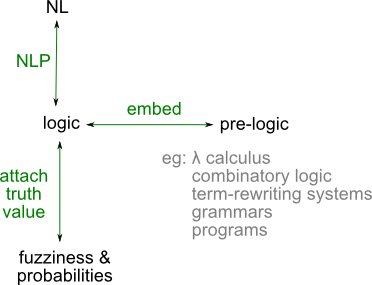
\includegraphics[scale=0.7]{prelogic.png}
% \caption{Prelogic}
\end{figure}
NL should be translated into logic because logic is closer to NL than pre-logic.  What really distinguishes ``logic'' from pre-logic is the notion of \textbf{propositions}, which is a unit of meaning to which we can attach \textbf{truth values}.  A proposition such as \formula{male(john)} is a ``complete'' entity of meaning, as opposed to the predicate \formula{male} which is incomplete, or ``syncategorematic''\footnote{The term syncategorematic has several meanings, here I mean any component of a sentence that is not a proposition.}.  This distinction is important because fuzziness and probabilities should be assigned to the logic rather than pre-logic.

The problem with the above configuration is, if the pre-logic is fixed and the logic is allowed to be dynamically learned, then it may be difficult to work with such a dynamically changing logic, in particular to assign fuzzy-probabilistic truth values to it, or to translate NL to it.

\section{Uncertainty}

Reasoning under uncertainty is a vast and nightmarishly complex topic in AI.  Simon Parsons's book \citep*{Parsons2001} contains a very good survey of uncertain reasoning, but even that is not exhaustive.  We may look at the following taxonomy of ``ignorance'' proposed by \citep*{Bosc1997}:
\begin{figure}[H]
\centering
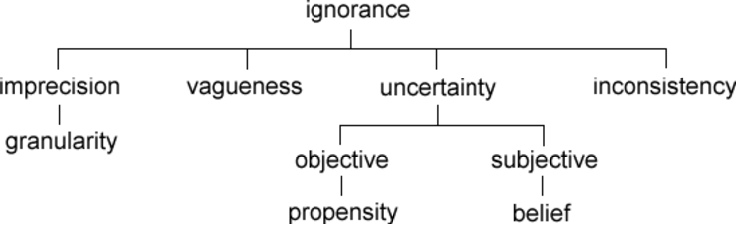
\includegraphics[scale=0.7]{IgnoranceTaxonomy.png}
\caption{taxonomy of ignorance}
\end{figure}

At first blush, classical logic appears to be sufficient for AGI.  Some AGI designers prefer to use crisp logic as the base and plan to build $\mathcal{P}$ and $\mathcal{Z}$ upon crisp logic.  But this may be a sign of not facing problems and not having sufficient understanding of fuzzy-probabilistic logics.  To represent $\mathcal{P}$ and $\mathcal{Z}$ logic \textit{in} crisp logic is like writing an entire $\mathcal{P}$-$\mathcal{Z}$ inference engine in Prolog, complicated by the fact that the crisp logic would be somewhat different from Prolog and so may be even harder to program in.  Also, the ``truths'' known by the AGI will then be different from the truths as represented in the crisp logic --- the former would be ``floating'' above the latter;  This creates unnecessary indirectness.  I will give other reasons in \S\ref{sec:whyZ} and \ref{sec:whyP}.

\textbf{Why not include other uncertainty measures besides $\mathcal{P}$ and $\mathcal{Z}$?}

There are other theories of uncertainty, such as possibility, belief functions, and rough sets.  The reason I chose $\mathcal{P}$ and $\mathcal{Z}$ is because they are simple and best understood.  There has been attempts to create systems where the user can create a flexible number of uncertainty measures, but one problem of such systems has been pointed out in \citep*{Parsons2001}:  If we have 3 uncertainty measures, say ``cloud'', ``mist'', and ``fog'', there would be a need to provide mixed inference rules for ``cloud-mist'', ``cloud-fog'' etc, a total of $n^2$ possibilities.  I have worked out the combination of $\mathcal{B}$, $\mathcal{P}$ and $\mathcal{Z}$ and found that it involved considerable efforts.

\section{Nonmonotonicity and defeasible reasoning}
\label{sec:exceptions}

One can create defeasible logics from classical logic, for example Reiter's \textbf{default logic} and McCarthy's \textbf{circumscription}.  But the classical approaches seem to require enumerating all possible exceptions, which is impractical.

\textbf{2 examples:}

\textbf{A.}\\
\textit{
1. John is usually very punctual.\\
2. Therefore, John will arrive at the airport on time.\\
3. John has an accident en route to the airport, and dies.\\
4. Therefore, John will NOT arrive on time.\\}
Will John arrive on time?

\textbf{B.}\\
\textit{
1. Mary has cybersex with many partners.\\
2. Cybersex is a kind of sex.\\
3. Therefore, Mary has many sex partners.\\
4. A person who has many sex partners has a high chance of STDs.\\
5. Therefore, Mary has a high chance of STDs.}

What's wrong with example B?  On the one hand, we should admit that cybersex is sex (it is a borderline case), but it lacks certain prominent features of sex, such as physical contact (which is not necessarily a \textit{defining} feature of sex).  Thus, if we carry on reasoning with the idea that cybersex is sex, we may get unsound conclusions.  The key to resolving this problem is to recognize ``cybersex is sex'' with \textbf{qualifications} such as ``it is sex without physical contact''.

If we have a rule that ``sex transmits certain diseases'', we may have to attach the exception ``only if the sex involves physical contact''.  In the end, our rules may be inundated with possibly infinitely many exceptions.  How can we get out of this problem?

\citep*{Wang1994}, \citep*{Wang2006} in NARS provided a solution.  His idea is not to store the exceptions to rules, but instead allow a \textit{multitude} of rules to fire, calculate the ``confidence'' (\S\ref{sec:confidence}) of each conclusion, and pick the conclusion with the highest confidence.  This allows us to handle exceptions relatively easily.

For the example:
\begin{eqnarray}
X \PimpL A \nonumber \\
X \PimpL B \nonumber
\end{eqnarray}
Pei Wang's idea is to calculate the combined conditional probability by weighing each individual conditional probability with their associated \textbf{confidences} (\S\ref{sec:confidence}):
$$ P(X|A,B) = \frac{ P(X|A)c_A + P(X|B)c_B }{ c_A + c_B } $$
which is a nice idea\footnote{Except that NARS truth values do not conform to probability theory.}, but Abram Demski came up with an alternative idea that is more in accord with Bayesianism.  The idea is to reconstruct $P(X|A,B)$ from the marginal conditionals $P(X|A)$ and $P(X|B)$ and priors $P(A)$ and $P(B)$.  This is achieved by applying Bayes' rule twice:
\begin{eqnarray}
P(X|A,B) &=& \frac{P(A,B|X)P(X)}{normalization} \nonumber \\
         &=& \frac{P(A|X)P(B|X)P(X)}{normalization} \nonumber \\
         &=& \frac{P(X|A)P(A)P(X|B)P(B)}{P(X) \; normalization}
\end{eqnarray}

\{ To-do:  Abram's solution seems problematic, I'm discussing it with him... \}

\section{Equality}
\index{equality}  \index{identity|see{equality}}
\label{sec:equality}

A problem with equality is illustrated by the classic example ``Morning Star / Evening Star''.  This is a similar example and its rendition in logic:\\
\tab
\begin{tabular}{l|l}
\textit{``Clark Kent is Superman.''}               & \formula{clark-kent = superman} \\
\textit{``Superman can fly.''}                     & \formula{can-fly(superman)} \\
\textit{``Mary does not know that Clark Kent is Superman.''} & $\neg$ \formula{know(mary, "clark-kent = superman")} \\
\textit{``Mary knows that Superman can fly.''}     & \formula{know(mary, can-fly(superman))} \\
\textit{``Mary does not know that Clark Kent can fly.''} & $\neg$ \formula{know(mary, "can-fly(clark-kent)")}
\end{tabular}

Perhaps the solution is that \formula{"clark-kent"} (in quotes, ie, the Clark Kent that Mary knows) is not equal to \formula{clark-kent} (without quotes, ie, the real Clark Kent).

\section{Modal logic}
\begin{flushright}
\emph{Modality, si! Modal logic, no!}\\
--- John McCarthy
\end{flushright}

My view is to use predicates to represent modality instead of using modal logics.  This view was first advocated by \citep*{McCarthy1997}.

One argument for the use of modal logic arises from the previous example:\\
\begin{tabular}{l|l}
\hspace*{1cm} \textit{``Mary believes Superman is dead.''} & \formula{believe(mary, dead(superman))}\\
\hspace*{1cm} \textit{``Superman is Clark Kent.''} & \formula{superman = clark-ken}\\
\hspace*{0.7cm} * \textit{``Mary believes Clark Kent is dead.''} & \formula{believe(mary, dead(clark-ken))}
\end{tabular}\\
but Mary may not know that Superman is Clark Kent.  This problem can be resolved as in the last section (\S\ref{sec:equality}).

\section{Shortcomings of the current logic}

1.  \textbf{Binary vs $\mathcal{P/Z}$.}  It may be desirable to have binary logic alongside $\mathcal{P/Z}$ logic.  $\mathcal{P/Z}$ reasoning is suitable for common-sense concepts, whereas binary reasoning is good for \textit{programmatic}
\footnote{Ie, binary logic makes programming easier}
or computational reasons.  However, one unsolved problem is that many common-sense concepts appear to be binary but are fuzzy upon close inspection (eg male/female, dead/alive).  The question is how to let binary and fuzzy concepts coexist in the same logic.

2.  \textbf{First-order vs Higher-order logic.}  Let us admit outright that FOL as a KR scheme is insufficient for common-sense reasoning and thus AGI.  But I also have the impression that second-order logic would be sufficient for most common-sense reasoning purposes.

With some tricks (such as reification, \S\ref{sec:reification}), FOL may be able to deal with second-order reasoning.

Another trick is that the FOL reasoner can ``escape'' to a meta-reasoner when higher-order constructs are needed.  This will be taken up on the chapter on meta-reasoning, \S\ref{ch:meta-reasoning}.

As a more satisfactory long-term solution, we are currently working on creating a $\mathcal{P(Z)C}$ HOL, see \S\ref{sec:HOL}.

%With P and Z, the AGI can express ideas such as:\\
%\hspace*{1cm} ``Mary is \underline{probably} \underline{fairly} tall.''

\section{$\mathcal{B}$: binary logic}
\label{sec:binary-logic}

My intuition is that common-sense reasoning involves mainly $\mathcal{B}$, followed by $\mathcal{Z}$, and $\mathcal{P}$ is relatively rare.

%Horn clauses:  P and Z rules can be expressed in Horn form only.  But it seems that we can use general resolution for B rules, no?  Or, perhaps I want to use something similar to Horn resolution for P and Z?

%Each rule will enable one inference step, so the logic is almost truth-functional.  The problem is the intermediate results... I only know how to do that in B form.  Maybe we can keep a set of disjunctions of truth values?

%In B logic the proof procedure keeps a current clause / or a line of clauses.  In Bayes net we have a query variable and the algorithm finds its P value.  Z logic may be similar to B logic because it's truth functional?

%Perhaps we can work out the general case of a query variable of any TV type?  If we draw a B rule that's easy.  If Z rule, then we have a few Z variables as goals.  They need Z rules to fulfill, but what if we have a B rule for one of the sub-goals?  Then we need to translate the B value to Z value.  We can only do that via P(Z).  So we have a P(Z) value as one of the subgoals.  This may cause the head of the rule to become P(Z) too.  It seems there is a tendency for all TVs to become P(Z).
%That will actually back-propagate along the proof sequence.

%Things may be even worse for a P rule.  The application of the rule requires other numbers.  

\section{Meta-reasoning}
\begin{flushright}
\emph{I think I think, therefore I think I am.}
\end{flushright}

The term ``meta-reasoning'' may refer to 2 things:\\
1. The ability to \textbf{reason about reasoning}, which is what this chapter is concerned with;\\
2. Scheduling reasoning tasks to achieve best results with limited computational resources (I have not thought about this problem yet).

An excellent survey of meta-reasoning in the \#1 sense is \citep*{Constantini2002}.

In the Tell-Learn loop, we see that we need a special predicate credible() to increase the probability of a statement via a side-effect.  But that may not be the only meta-reasoning move we can make.

Another example is the $B \leftrightarrow Z$ conversion of ``traitor'' and ``patriot'' (\S\ref{sec:PZ-meta-reasoning}).

\section{Higher order logic}
\label{sec:HOL}

The HOL formulation that I am most familiar with is \citep*{Lloyd2003}.  It uses \textbf{typed lambda calculus} to represent logical formulae.  This representation is specifically developed for use as a logic programming language (Escher) and for inductive learning.

Interestingly, Lloyd uses a form of algebraic logic that is similar to what I do with $\mathcal{P(Z)C}$ logic, ie, its statements are of the form $H = B$ where $H$ is the head and $B$ is the body.  In essence this is the Prolog / Horn tradition.

\{ TO-DO:  formulate a $\mathcal{P(Z)C}$ HOL \}

\label{sec:PZ-meta-reasoning}

One example of meta-reasoning pertinent to fuzziness is:\\
\hspace*{1cm} S1: ``You are either a patriot or a traitor.''\\
\hspace*{1cm} S2: ``No, I can be slightly patriotic or slightly traitorous.''

In S1 the predicates \textit{patriot} and \textit{traitor} have binary character.  In S2 they have fuzzy character.

\underconst


\chapter{Inference}
\label{ch:inference}
\begin{flushright}
\emph{A syllogism has 3 parts; therefore, this is not a syllogism.}
\end{flushright}
\minitoc

By inference we mean deduction and abduction;  induction is regarded a form of learning.

What are the computational bottlenecks?  How to speed things up?

\section{Some background}

\subsection{Resolution}
\label{sec:resolution}

\subsection{Horn clauses and Prolog}

\subsection{Forward- and backward- chaining}

\subsection{Complexity of inference}

Some facts:

1.  Satisfiability in binary \textbf{first-order logic} is semi-decidable (ie, it terminates in finite time if a proof exists, but may never terminate if a proof does not exist)

2.  SAT for binary \textbf{propositional logic} is NP-complete.

3.  \textbf{Propositional Bayesian network} inference is \#P-complete (ie, it is as hard as returning the number of solutions to an NP-complete problem).

4.  The \textit{naive} algorithm for propositional Bayesian network inference is $O(n 2^n)$ where $n$ is the number of nodes.

5.  Pearl's message-passing algorithm is an \textit{exact} algorithm for propositional Bayesian network inference;  therefore it also requires non-polynomial time in the worst case.

6.  Pearl's algorithm, when operating on trees, is linear time.  But trees seem to be insufficient for AGI reasoning.

7.  SAT for the \textbf{propositional Horn} subclass of binary logic, can be performed in linear time.  My very simple algorithm for Bayesian inference is analogous to Horn deduction\footnote{The term Horn can only be used to describe binary logic:  a Horn clause is a clause with exactly one positive literal.  $\mathcal{PZ}$ logic has a Horn-like form, but the distinction between positive and negative literals disappears in logics with numerical truth values.}.  Prolog owes its efficiency to SLD resolution which is also Horn-based.

\section{Nonmonotonicity and redundancy}

\subsection{Handling exceptions (nonmonotonic reasoning)}
\label{sec:exceptions}

Fuzzy reasoning can sometimes lead to unsound conclusions, for example:\\
\textit{1. Mary has cybersex with many partners.\\
2. Cybersex is a kind of sex.\\
3. Therefore, Mary has many sex partners.\\
4. A person who has many sex partners has a high chance of STDs.\\
5. Therefore, Mary has a high chance of STDs.}

What's wrong with this example?  On the one hand, we should admit that cybersex is sex (it is a borderline case), but it lacks certain prominent features of sex, such as physical contact (which is not necessarily a \textit{defining} feature of sex).  Thus, if we carry on reasoning with the idea that cybersex is sex, we may get unsound conclusions.  The key to resolving this problem is to recognize ``cybersex is sex'' with \textbf{qualifications} such as ``but it is sex without physical contact''.

If we have a rule saying that ``sex transmits certain diseases'', we may have to attach the exception ``only if the sex involves physical contact''.  In the end, our rules may be inundated with possibly infinitely many exceptions.  How can we get out of this problem?

\citep*{Wang1994}, \citep*{Wang2006} provided a solution, which I essentially adopt.  His idea is not to store the exceptions to rules, but instead allow a \textit{multitude} of rules to fire, calculate the ``confidence'' (\S\ref{sec:confidence}) of each conclusion, and pick the conclusion with the highest confidence.  This allows us to handle exceptions relatively easily.

%Another example:\\
%\hspace*{1cm} \textbullet \textit{ Penguins are birds but they cannot fly.}

%``Nonmonotonic'' means that, when you add a statement to a KB (knowledgebase), some of the earlier conclusions of the KB may no longer be valid.

%For example, you may have a Prolog rule that says:\\
%\hspace*{1cm} \ttfamily fly(X) :- bird(X). \rmfamily\\
%but you may also add an \emph{exception} to this rule:\\
%\hspace*{1cm} \ttfamily fly(X) :- penguin(X), !, fail. \rmfamily\\
%which means that if penguin(X) is true, fly(X) would fail.\\
%The application of the second rule...

%\subsection{Doing B inference as Z inference}

%TO-DO:  There is a possibility of performing all reasoning in pure $\mathcal{Z}$-logic.  Might it be more advantageous than a hybrid $\mathcal{BPZ}$ logic...?

%$patriot \curlyvee traitor = 0.8$\\
%$\neg patriot \Rightarrow z(patriot) = 0.25$

\section{Deduction}
\label{sec:deduction}

%\subsection{$\mathcal{Z}$ inference algorithm}
%\label{sec:pureZinference}
%
%\{ TO-DO:  The inference algorithms can be made much simpler if we adopt the idea of the Horn form in binary logic. \}
%
%$\mathcal{Z}$ inference (Algorithm \ref{algorithm1}) is analogous to backward-chaining in binary logic (such as Prolog), except that it calculates the $\mathcal{Z}$ value of the query.
%
%\begin{algorithm}
%\caption{backward-chaining Z inference}
%\label{algorithm1}
%\begin{algorithmic}[1]
%
%\REQUIRE a knowledgebase $KB$, a list of query goals $G$ \\
%\ENSURE $z =$ the truth value of $G$.
%
%\REPEAT
%	\STATE choose a literal $L$ from the list $G$, removing it from G
%	\STATE find a rule $z_0 := \widetilde{\bigvee} \widetilde{\bigwedge} z_{ij} $ such that\\
%			 $L$ unifies with the consequent $z_0$ \\
%	\COMMENT{ if $z_{ij}$ is null, $z_0$ is a fact in $KB$ }
%	\STATE add the rule's antecedents ($z_{ij}$) to the list $G$ \\
%	\STATE if depth of recursion $< h$ \\
%			 recurse to resolve the new list of goals $G$ \\
%\UNTIL{ there are no more applicable rules in $KB$. }
%
%\end{algorithmic}
%\end{algorithm}

\subsection{$\mathcal{P}$ inference algorithm}
\label{sec:P-inference}

%The $\mathcal{P}$ inference algorithm is similar to $\mathcal{Z}$ inference (Algorithm \ref{algorithm1}) except that probabilistic inference can be ``abductive'' --- a conditional probability can work in the reverse direction via Bayes theorem --- thus the branching factor of the search would be higher.
%
%\begin{algorithm}
%\caption{backward-chaining P inference}
%\label{algorithm2}
%\begin{algorithmic}[1]
%
%\REQUIRE a knowledgebase $KB$, a list of query goals $G$ \\
%\ENSURE $p =$ probability of $G$.
%
%\REPEAT
%	\STATE choose a literal $L$ from the list $G$, removing it from G
%	\STATE find a rule $X_0 \leftarrow \bigcurlyvee \bigcurlywedge X_{ij} $ such that\\
%			 $L$ unifies with one of the $X_{ij}$'s, including $X_0$\\
%	\COMMENT{ if $X_{ij}$ is null, $X_0$ is a fact in $KB$ }
%	\STATE add the $X$'s to the list $G$, except the one that unifies with $L$ \\
%	\STATE if depth of recursion $< h$ \\
%			 recurse to resolve the new list of goals $G$ \\
%\UNTIL{ there are no more applicable rules in $KB$. }
%
%\end{algorithmic}
%\end{algorithm}

TO-DO: Deal with loops.

TO-DO: There should be a mechanism to prune low-probability (or should it be low-confidence?) branches early on in the search.

TO-DO: Compare $\mathcal{P}$ inference with standard Bayesian network inference algorithms...?\\
This algorithm merely outlines the rules involved in computing $P(X)$.

Problems of Bayesian network inference:\\
1.  Some inference steps analogous to classical logic cannot be performed because probabilities are not truth-functional (ie, the probability of a statement is not the function of the probabilities of its constituents; it may depend on other probabilities not appearing in the statement).\\
2.  Bayesian network inference cannot be performed one-rule-per-step because of interdependence of variables that requires message passing.

Currently I am using an extremely simplified approximation.

%The solution to \#1 is to use 0.5 as the substitute for unknown probabilities.

%The solution to \#2 is to use only local dependencies.

%Case \#1:
%\begin{figure}[H]
%\centering
%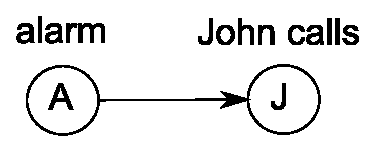
\includegraphics{BayesNet-alarm-John.eps}
%\end{figure}
%\textbf{Forward inference}: the answer is simply what is given: $P(J|A)$\\
%\textbf{Backward inference (abduction)}: we seek $P(A|J)$ which is given by Bayes rule:\\
%$$ P(A|J) = \frac{P(J|A)P(A)}{P(J)} $$
%and we search for values of $P(A)$ and $P(J)$; If they don't exist we substitute with 0.5.

%It seems that we need to record the rule during inference.  When the subgoals are all found we can obtain the head.  Is there a way not to store the rules?  No.  Not only that, but we need to have backtrack ability too.

%Case \#2:
%\begin{figure}[H]
%\centering
%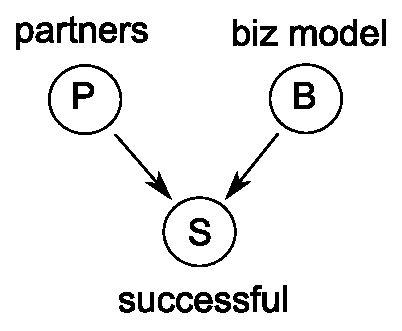
\includegraphics{BayesNet-successful-business.eps}
%\end{figure}
%\textbf{Forward inference}: simply given by $P(S|P,B)$\\
%\textbf{Abduction}: given S, we can infer P and B.  "P or B" is a problem. How to represent that?  

\subsection{Hybrid $\mathcal{B,P,Z}$ inference}

Rules, which are the building blocks of inference, can be of 4 types:

\begin{table}[H]
\parbox{3cm}{\caption{}}
\begin{tabular}{|l|l|} \hline
\multicolumn{2}{|c|}{\textbf{rules}}\\ \hline
mnemonic                   & meaning\\ \hline
$\mathcal{B}$              & Prolog statements of the form\\
                           & \qquad $L_0 \, \mbox{:--} \, L_1, L_2, L_3, ... $ \\
$\mathcal{Z}$              & Fuzzy rules of the form\\
                           & \qquad $z_0 := \widetilde{\bigvee} \; \widetilde{\bigwedge} \; z_{ij}$ \\
$\mathcal{P(B)}$           & Bayesian network nodes specified by\\
                           & \qquad $X_0 := \bigcurlyvee \bigcurlywedge X_{ij};c_{ij}$ \\
$\mathcal{P(Z)}$           & Specifications of $\mathcal{P(Z)}$ distributions\\
                           & \qquad $X_0 := Beta(\mu,\sigma^2)$ \\
\hline
\end{tabular}
\end{table}

In principle, a unified form of $\mathcal{P(Z)}$ rule is possible, but I have found it to be too complex and unwieldy to use.  So we will use a hybrid mixture of the above 4 types of rules.

%P(Z) rules:  I can specify the mean and variance of the distribution for a variable.  Or, I can specify the mean or variance only.

The type of a rule is determined by its ``head'' --- eg, if the head is a $\mathcal{B}$ variable then the rule is a $\mathcal{B}$ rule.  Using unified $\mathcal{P(Z)}$ truth values, we can plug variables of any TV type into any rule.  So, the rule type only affects how the rule is interpreted, which will be explained below.

%A rule may involve factors of TV types other than its own TV type, which is handled by Table \ref{table:TV-rules-combinations}.

An example of a rule is:  ``almost Q'' means ``close to Q, but not being Q''.\\
The TV types of the predicates are:\\
\hspace*{1cm} ``almost Q'' --- $\mathcal{B}$\\
\hspace*{1cm} ``close to Q'' --- $\mathcal{Z}$\\
\hspace*{1cm} ``not Q'' --- $\mathcal{B}$\\
So we can represent it with a $\mathcal{B}$ rule:\\
\hspace*{1cm} $\mbox{almost } Q \leftarrow \mbox{ close-to } Q \wedge \neg Q$
Despite using a $\mathcal{B}$ rule, the result of inference will be a $\mathcal{P(Z)}$ truth value with binary character.  This is a good thing, because the idea of ``almost'' can be fuzzy in some cases, for example:\\
\hspace*{1cm} ``I heard that John almost got killed by the assassination?''\\
\hspace*{1cm} ``Not really, the bullet only hit his toe!''

%where the head is of type $\mathcal{B}$, the first factor is of type $\mathcal{Z}$, the second factor is of type $\mathcal{B}$.

%In general, inference proceeds by drawing rules from the KB.  Conclusions of various TV types will be generated depending on the TV type of the rules being applied.

To simplify things, I consider single inference steps.  A complete proof involves a series of such steps.

\subsubsection{$\mathcal{B}$ rule:}

The $\mathcal{B}$ rule can have 3 operators: $\wedge$, $\vee$, and $\neg$.  All we need to do is to show how to evaluate the operators for $\mathcal{P(Z)}$ values.  An example $\mathcal{B}$ rule is:\\
\hspace*{1cm} \texttt{bachelor :- male $\wedge \; \neg$ married}

Case $\neg$ :  We need to convert the $\mathcal{P(Z)}$ distribution to one with a binary character.  This is done by setting the variance to a fixed value in the binary regime (\S\ref{sec:unifying-P(Z)}).  Then the result is negated by transforming the mean:
\begin{equation}
\mu ' = 1 - \mu
\label{eqn:1-minus-z-transform}
\end{equation}

Case $\wedge$ : Convert the $\mathcal{P(Z)}$ value to $\mathcal{P(B)}$ via eqn (\ref{eqn:mean-and-p}).  Then $P(A \wedge B) = P(A) P(B)$, assuming independence.

The variance is assigned a fixed value so that the resulting variable has binary character.  Note that the resulting variance is not affected by the variances of the premises because the aim of a $\mathcal{B}$ rule is to form a \textit{binary} judgment.

Case $\vee$ : Similar to above, with $P(A \vee B) = P(A) + P(B) - P(A)P(B)$, again assuming independence.

\subsubsection{$\mathcal{Z}$ rule:}

$\mathcal{Z}$ rules can have the operators $\widetilde{\wedge}$ (= min), $\widetilde{\vee}$ (= max), $\widetilde{\neg}$ ($= 1-z$) and the fuzzy modifier $\Gamma()$.  At this stage we ignore Soft min and max.  The $\Gamma()$'s are applied before the other operators.

Case $\Gamma$() : If $z_0 := \Gamma(z_1)$ and $z_1$ is given by the probability density function $f_1(z1)$, then the probability density of $z_0$ would be given by:
\begin{equation}
f_0(z_0) = f_1(\Gamma^{-1}(z_0)) \left | \frac{d\Gamma^{-1}}{dz_0} \right |
\end{equation}
which is explained in \citep*{Wikipedia2008}.  If $\Gamma()$ is the Gaussian function given in eqn (\ref{eqn:fuzzy-moderator-Gaussian}) then\\
$$ f_0(z_0) = f_1(\pm \sigma \sqrt{-2 \ln z_0} + z^*) \left | \frac{\sigma}{z_0 \sqrt{-2 \ln z_0}} \right | $$
but there is a glitch:  $\Gamma^{-1}()$ has 2 pieces, and their contributions must be summed up piecewise.  Sometimes the resulting distribution looks irregular, for example:
\begin{figure}[H]
\centering
\includegraphics[scale=0.9]{Z1-Gaussian-transform-to-Z0-ugly.ps}
\end{figure}
but we can approximate it with a Beta distribution by preserving the mean and variance.  The irregular appearance does not matter that much if we only care about the mean and variance.  I have obtained the approximation formula by numerical integration and nonlinear regression on randomly generated samples, as follows ($m_1$ = mean of input, $m_0$ = mean of result):
\begin{figure}[H]
\centering
\includegraphics[scale=0.7]{Gaussian-fuzzy-modifier-regression-result.ps}
\caption{Gaussian fuzzy modifier:  empirical data and result of regression}
\end{figure}

Case $\neg$ :  Simply negate the $\mathcal{P(Z)}$ distribution by eqn (\ref{eqn:1-minus-z-transform}) with variance unchanged.

Case $\widetilde{\vee}$ :  Given $z_0 := z_1 \widetilde{\vee} z_2$, ie $z_0 = max(z_1, z_2)$.  What we need to do here is to calculate the PDF of a random variable given as a function of two other random variables.  The procedure is given in many textbooks.

Here $\mathbf{P}$ denotes probability measure which is a set function, $F(t)$ denotes CDF's, $f(t)$ denotes PDF's.

%Define the region $D_0 := \{ (z_1,z_2): \widetilde{\wedge}(z_1,z_2) \leq z_0 \}$.
%\begin{eqnarray}
%F_0(z_0) & = & \mathbf{P}(Z_0 \leq z_0)\\
%         & = & \mathbf{P}((Z_1,Z_2) \in D_0)\\
%         & = & \iint_{D_0} f_{12}(z_1,z_2) dz_1 dz_2
%\end{eqnarray}
%If we assume $Z_1, Z_2$ independent then $f_{12}(z_1,z_2) = f_1(z_1) f_2(z_2)$.

\hspace*{1.2cm} $ F_0(t) = \mathbf{P}(Z_0 \leq t)$\\
\hspace*{2cm} $= \mathbf{P}(\widetilde{\vee}(Z_1,Z_2) \leq t)$\\
\hspace*{2cm} $= \mathbf{P}(max(Z_1,Z_2) \leq t)$\\
\hspace*{2cm} $= \mathbf{P}(Z_1 \leq t \wedge Z_2 \leq t)$\\
\hspace*{2cm} $= \mathbf{P}(Z_1 \leq t) \, \mathbf{P}(Z_2 \leq t)$ \quad assuming $Z_1, Z_2$ independent\\
\hspace*{2cm} $= F_1(t) F_2(t)$\\
where $$ F_1(t) = \int_0^t f_1(z_1) dz_1 , \quad F_2(t) = \int_0^t f_2(z_2) dz_2$$

%The result we want is: $ f_0(t) = dF_0(t) / dt $
The result we want is:
\[ f_0(t) = \frac{dF_0(t)}{dt} = F_2(t) \frac{dF_1(t)}{dt} + F_1(t) \frac{dF_2(t)}{dt} \]
and we need to apply Leibnitz's Rule.\footnote{For a function of t defined by: $$ F(t) := \int_a(t)^b(t) \Phi(x,t) dx $$ its differentiation is given by Leibnitz's Rule: $$ \frac{dF(t)}{dt} = \int_{a(t)}^{b(t)} \frac{\partial\Phi(x,t)}{\partial t} dx + \Phi(b(t),t) \frac{db(t)}{dt} - \Phi(a(t),t) \frac{da(t)}{dt} $$ }  Then we get:
\begin{equation}
f_0(t) = f_1(t) F_2(t) + f_2(t) F_1(t)
\end{equation}

%If it is $min()$:\\
%\hspace*{1.2cm} $ F_0(t) = \mathbf{P}(\widetilde{\vee}(Z_1,Z_2) \leq t)$\\
%\hspace*{2cm} $\approx \mathbf{P}(min(Z_1,Z_2) \leq t)$\\
%\hspace*{2cm} $= \mathbf{P}(Z_1 \leq t \vee Z_2 \leq t)$\\
%\hspace*{3cm} assuming $Z_1, Z_2$ independent:\\
%\hspace*{2cm} $= \mathbf{P}(Z_1 \leq t) + \mathbf{P}(Z_2 \leq t) - \mathbf{P}(Z_1 \leq t) \mathbf{P}(Z_2 \leq t)$\\
%\hspace*{2cm} $= F_1(t) + F_2(t) - F_1(t) F_2(t)$

This function $f_0$ has an interesting property:  it appears to add up the distributions $f_1$ and $f_2$, \textit{with the one on the right being dominant}, ie, giving the biggest contribution of probability mass (or area under the curve).  Some examples are as follows:
\begin{figure}[H]
\centering
\includegraphics[scale=0.8]{A-ZOR-B-examples.ps}
\caption{$z_0 := z_1 \, \widetilde{\vee} \, z_2$}
\end{figure}

%Again, the resulting distribution $f_0(z_0)$ may have an irregular shape, for example:
%\begin{figure}[H]
%\centering
%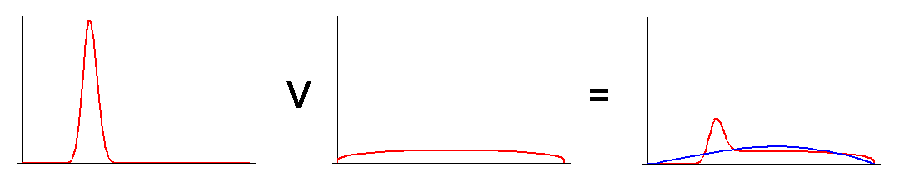
\includegraphics[scale=1.0]{A-max-B--ugly-pdf.eps}
%\caption{pdf's of $z_1$, $z_2$, $max\{z_1,z_2\}$}
%\end{figure}
%where the blue line is the Beta distribution approximation (made by preserving the mean and variance).

%Some observations about the shapes:
%
%A. When the 2 inputs are unimodal:
%
%1. If they are narrow (ie small variance) and fairly separated, the mode on the right almost completely dominates; deviation is negligible.\\
%2. When the 2 modes are close, the mean of the result shifts to the right and variance decreases (the peak gets narrower).\\
%3. If any one input is broad (ie large variance), the result will shift to the right.  The change in variance is ambiguous.
%
%new mean = right mean + (amount of shift)
%amount of shift = f( how close they are, how broad they are)
%if close then new variance = narrower
%
%B. When 1 of the inputs has infinity on one side or both:
%
%1. If infinity is on both sides, the result will retain the infinity on the right, plus a small second peak near the second input (which is shifted slightly to the right).  It may be approximated by a J shape with a or b = 1 on one side.\\
%2. If infinity occurs on the right only (J shape), that infinity dominates the result, and the second input has a rather slight effect.\\
%3. If infinity occurs on the left, the second input will dominate.  Deviation from the second input is very slight.
%
%C. If both inputs have infinities:
%
%1. When 2 J shapes are crossed, the right side dominates, and there is a very slight shift to the left (but the stats seem to indicate that the shift can be big).  Sometimes, but rarely, to the right too -- why? Well the reason can be quite obscure.\\
%2. With a U shape and a J shape to the left, the result is a J shape to the right but with a small peak near the left end.  May be difficult to approximate (or use the power distribution?)\\
%3. With a U shape and a J shape to the right, the result is a J shape to the right with a greater variance (ie more polarized).  The degree of extra polarization depends on the contribution of the U shape (whether it's heavy on the right side).\\
%4. With 2 U shapes, the result is a J shape.

Once again, we approximate by preserving the mean and variance; The irregular appearance is not so important.  By looking at the following graph we can see that the mean of the result ($m_0$) is mostly dominated by $m_2$ which is the mean of the input further to the right (ie, $m_2 > m_1$).  There is sometimes a slight shift to the right relative to $m_2$ (the dots above the $x=y$ line), but it seems insignificant and may be ignored.  In other words, the fuzzy inference rule is very simple:  \textit{the mean of the result is just the greater mean of the 2 inputs}.  A similar graph shows that the variance of the result is also approximately equal to the variance of the rightmost input.
\begin{figure}[H]
\centering
\includegraphics[scale=0.8]{z1-OR-z2-M-and-V-plots.ps}
\caption{Plots of mean and variance; output vs input}
\end{figure}

%Divide into 16 cases...
%\begin{figure}[H]
%\centering
%\includegraphics[scale=0.8]{z1-OR-z2-10-cases.ps}
%\caption{10 cases for $Z1 \widetilde{\vee} Z2$}
%\end{figure}

Case $\widetilde{\wedge}$ : The result for $z_0 := z_1 \, \widetilde{\wedge} \, z_2$ is similar (again assuming $Z_1, Z_2$ independent):
\begin{equation}
f_0(t) = f_1(t) + f_2(t) - f_1(t) F_2(t) + f_2(t) F_1(t)
\end{equation}

In summary, the fuzzy inference rules are:

\fbox{ \parbox{7cm}{
1. For $z_0 := \Gamma(z_1)$,
$$ \mu_0 = \frac{k_1+k_2}{\sigma_1} e^{- (m_1-z^*)^2 / \sigma_1^2 } $$
$$ v_0 = \frac{k_3}{\sigma_2} e^{- (z^* - \sqrt{3} m_1 + k_4)^2 / \sigma_2^2 } $$
\hspace*{0.3cm} where $\sigma_1 = k_1 (m_1+z^*-1)^2 + k_2 $ \\
\hspace*{1.4cm}     $\sigma_2 = k_5 (z^* + \sqrt{3} m_1 - k_6)^2 + k_7 $ \\
\hspace*{0.3cm} and the $k$'s are regression parameters\\
2. For $z_0 := \neg z_1$, $\mu_0 = 1 - \mu_1$, $v_0 = v_1$ \\
3. For $z_0 := z_1 \widetilde{\vee} z_2$ or $z_1 \widetilde{\wedge} z_2$, \\
\hspace*{0.3cm} $\mu_0 = max(\mu_1, \mu_2)$ or $min(\mu_1, \mu_2)$, \\
\hspace*{0.3cm} $v_0 = v_1$ or $v_2$ following the choice above
}}

\subsubsection{$\mathcal{P(B)}$ rule:}

A $\mathcal{P(B)}$ rule is of the form:\\
\hspace*{1cm} $X_0 := \bigcurlyvee \bigcurlywedge X_{ij};c_{ij}$

To simplify things, we do not implement the Bayesian network algorithm, instead we only perform the calculation $X_0$ from $X_{ij}$ in one direction.  This is an extreme simplification of probability logic, but it may already be sufficient for common-sense reasoning.  We will try this first and see how far it can go.

The $\mathcal{P}(\mathcal{Z})$ variables can be converted to $\mathcal{P}(\mathcal{B})$ variables via eqn (\ref{eqn:mean-and-p}).  Then the $\mathcal{P(B)}$ value of the consequent can be obtained via straightforward application of probabilities, eg:\\
%\hspace*{1cm} $P(X_1 \wedge X_2) = \sum_{i=1,2} P(X_1 \wedge X_2 \; | \; P(X_i)) \; P(X_i)$ \\
\hspace*{1cm} $ P(X_1 \wedge X_2) = (1-p_1)(1-p_2)(1-c_1)(1-c_2) \; + $ \\
\hspace*{3.5cm} $ (1-p_1)p_2(1-c_1)c_2 \; + $ \\
\hspace*{3.5cm} $ p_1(1-p_2)c_1(1-c_2) \; + $ \\
\hspace*{3.5cm} $ p_1 p_2 c_1 c_2 $ \\
where $p_i = P(X_i)$.  Note that it reduces to the binary case when $c_1 = c_2 = 1$.  The result is then converted back as a $\mathcal{P(Z)}$ distribution (with binary character).

\subsubsection{$\mathcal{P(Z)}$ rule:}

We do not use truly $\mathcal{P(Z)}$ rules because they are too complex and not needed for common-sense reasoning.  The $\mathcal{P(Z)}$ rules we have are simpler operations that allow us to manipulate the $\mathcal{P(Z)}$ distributions of variables.

We can directly assign the mean and variance to a $\mathcal{P(Z)}$ variable:\\
\hspace*{1cm} $X_0 := Beta(z; a, b)$

Or we can fix the probability at a particular point $z*$'s neighborhood.  For example, ``the probability of Mary being 0.9 fat is 0.1''.

%\textcolor{red}{The stuff below this line are just my notes and may contain many errors.}
%\hrulefill

%In the probabilistic setting... we have to deal with adding rules and using the ``combination rule''... 
%
%\hspace*{1cm} \[ f = \frac{f_1 w_1 + f_2 w_2}{w_1 + w_2} \]

%The assumption is...?
%
%The confidence of the result is given by:\\
%\hspace*{1cm} \[ c = C(c_1, c_2) ? \]

%\subsection{Hybrid rules}
%\label{sec:hybrid-rules}
%
%Some rules may involve factors of various truth-value types.  For example, ``almost'' means ``close to, but not being'', which translates to this rule:\\
%\hspace*{1cm} $\mbox{almost } Q \leftarrow \mbox{ close-to } Q \wedge \neg Q$\\
%where the first factor is $\mathcal{Z}$, the second factor is $\mathcal{B}$.
%
%Maybe we should disallow $\mathcal{P}(\mathcal{Z})$-rules in the AGI because they are too sophisticated?
%
%The hybrid rules can be:\\
%\hspace*{1cm} \begin{tabular}{|l|l|l|l|l|} \hline
%                           & $\mathcal{B}$           & $\mathcal{Z}$                     & $\mathcal{P}(\mathcal{B})$ & $\mathcal{P}(\mathcal{Z})$\\ \hline
%                           & $\vee \wedge$           &                                   &            & \\
%$\mathcal{Z}$              & case H1                 & $\widetilde\vee \widetilde\wedge$ &                         & \\
%$\mathcal{P}(\mathcal{B})$ & $\curlyvee \curlywedge$ & case H2                           & $\curlyvee \curlywedge$ & \\
%$\mathcal{P}(\mathcal{Z})$ & case H3                 & case 8                            & case H4                 & $\widetilde\curlyvee \widetilde\curlywedge$ \\ \hline
%\end{tabular}
%
%TO-DO:  unfinished.

%\subsection{Unified $\mathcal{P(Z)}$ rules?}
%\label{sec:unified-BPZ-inference}
%
%This section is optional.  As far as inference goes, the rest of this chapter has outlined the algorithms.  Here we try to see how $\mathcal{B}$, $\mathcal{P}$, and $\mathcal{Z}$ can be unified under the most general logic, $\mathcal{P}(\mathcal{Z})$.  Such a logic may be desirable in machine learning, where the general form of $\mathcal{P}(\mathcal{Z})$-rules may allow us to perform the searching in a continuous space, and some of the rules will degenerate nicely into $\mathcal{B}$, $\mathcal{Z}$, and $\mathcal{P}(\mathcal{B})$ rules.  Anyway, it turns out that $\mathcal{P}(\mathcal{Z})$-rules are not that simple and degeneration is also complex.
%
%First, let's start with a general form of $\mathcal{Z}$-rule which is a function $\mathcal{Z} \times \mathcal{Z} \cdots \rightarrow \mathcal{Z}$:\\
%$$ z_0 := \widetilde{\bigvee_i}\, \widetilde{\bigwedge_j}\, \Gamma_{ij}(z_{ij}) $$
%where $\Gamma_{ij}$ are Gaussian functions with means $z^*_{ij}$ and variances $v_{ij}$ (in other sections we don't use the variance).  The interpretation of $\Gamma$ is:  $z^*_{ij}$ represent the optimal values, which results in $\Gamma = 1$, and when $z_{ij}$ deviates from $z^*_{ij}$, $\Gamma$ drops from 1.
%
%Now generalize this to the $\mathcal{P}(\mathcal{Z})$-rule which is a function $\mathcal{P}(\mathcal{Z}) \times \mathcal{P}(\mathcal{Z}) \cdots \rightarrow \mathcal{P}(\mathcal{Z})$.  Let's denote $\mathcal{P}(\mathcal{Z})$ variables as $\mathbf{W}$.  Each $\mathbf{W}$ is a Beta distribution with mean $z^*$ and variance $v$.  A $\mathcal{P}(\mathcal{Z})$-rule has the general form:\\
%\begin{equation}
%\mathbf{W}_0 \leftarrow \widetilde{\bigcurlyvee_i} \, \widetilde{\bigcurlywedge_j}\, \Gamma_{ij}(\mathbf{W}_{ij})
%\end{equation}
%which contains the parameters $z^*_{ij}$, $v_{ij}$, and $c_{ij}$ (from the probabilistic $\curlyvee \curlywedge$, \S\ref{sec:probabilistic-AND-OR}).  $\widetilde{\curlyvee} \widetilde{\curlywedge}$ is different from $\widetilde{\vee} \widetilde{\wedge}$ and $\curlyvee \curlywedge$, and the rule is interpreted as follows:
%
%\textbullet \, If the rule is $ \mathbf{W}_0 \leftarrow \Gamma_1(\mathbf{W}_1) $ we simply apply $\Gamma_1$ to the distribution $\mathbf{W}_1$.  The variance of $\mathbf{W}$ may change because of $\Gamma$.  This is covered in \hyperref[case8]{Case \#8}.
%
%\textbullet \, Suppose the rule is $ \mathbf{W}_0 \leftarrow \mathbf{W}_1 \, \widetilde{\curlyvee} \, \mathbf{W}_2 $.  In \hyperref[case8]{Case \#8} we considered how to plug a $\mathcal{P}(\mathcal{Z})$-variable into a $\mathcal{Z}$-rule.  There, the $\mathcal{Z}$-rule did not actively affect the probability distributions.  Now the $\widetilde{\curlyvee}$ adds a constraint on the probability of $\mathbf{W}_0$ based on the values $c_1, c_2$ (from eqn (\ref{eqn:probabilistic-AND-OR})).  So we add the constraint:\\
%\hspace*{1cm} $ P(z_0 = z^*_0 \, | \, z_1 = z^*_1, z_2 = z^*_2) = c_1 + c_2 - c_1 c_2 $\\
%where the RHS comes from eqn (\ref{eqn:probabilistic-AND-OR}).  The effect of this is to change the shape of $\mathbf{W}_0$ to ``sharper'' or ``broader''.  The sharper the shape, and thus the smaller the variance, the more certain we are that $z_0 = z^*_0$.  But the formula is incorrect because continuous probabilities at a point is meaningless.  So we need to say\\
%\hspace*{1cm} $ P(z_0 \in N(z^*_0) \, | \, z_1 \in N(z^*_1), z_2 \in N(z^*_2)) = c_1 + c_2 - c_1 c_2 $\\
%where N is the interval $[0,\frac{1}{2}]$ or $[\frac{1}{2},1]$, whichever $z$ is in, thus transforming $z$ as binary.
%
%\textbf{Degeneration of rules.}
%
%\textbullet \, A $\mathcal{P}(\mathcal{B})$-rule reduces to a $\mathcal{B}$-rule when $c_{ij} \rightarrow 1$ (\S\ref{sec:probabilistic-AND-OR}).\\
%\textbullet \, A $\mathcal{P}(\mathcal{Z})$-rule reduces to a $\mathcal{Z}$-rule when $c_{ij} \rightarrow 1$.\\
%\textbullet \, A $\mathcal{Z}$-rule reduces to a $\mathcal{B}$-rule when $\Gamma_{ij} \rightarrow I$, the identity function.\\
%\textbullet \, A $\mathcal{P}(\mathcal{Z})$-rule reduces to a $\mathcal{P}(\mathcal{B})$-rule when $\Gamma_{ij} \rightarrow I$.
%
%One problem is that when we say a $\mathcal{P}$-rule degenerates into a $\mathcal{B}$-rule, it can remain to be a $\mathcal{Z}$-rule with $\Gamma_{ij} = I$.  The rule itself cannot tell us which type it is.

\subsection{Inference of $\mathcal{C}$}
\label{sec:confidenceInference}

Confidence was introduced in \S\ref{sec:confidence}.  There, I explained that:\\
1. The confidence of rules can be measured in a frequentist way\footnote{Note, however, that the confidence c is not a frequency; it is just related to the frequency. }\\
2. The confidence of ground facts must be inferred

The problem is, we must initially know the confidence of at least \textit{some} ground facts in order to infer those of others.  To this end, I propose a convention to assign all \textbf{raw sensory events} (eg, ``a camera's pixel records the RGB color \#556677 at time 012345'')  to have confidence 1 (and thus $\infty$ support).  (It should not have 0 confidence because that would mean, informally, that the statement is so weak as to have no support at all).

In general, each inference step involves a rule of the form:\\
\hspace*{1cm} A $\longleftarrow$ B, C, D, ...\\
where the rule has a frequentist confidence $c_R$, and the antecedents B, C, D,... each has an inferred confidence.  So how to calculate $c_A$ from $c_B, c_C, c_D,$ ...?

Let's start from the simplest case.  Consider the rule:\\
\hspace*{1cm} A $\leftarrow$\textemdash\textemdash\textemdash\textemdash\textemdash $\,$ B\\
\hspace*{1cm} ? \hspace*{0.8cm} $c_R$ \hspace*{0.7cm} $c_1$ \\
where \hspace*{0.4cm} $c_R$ = confidence of the rule\\
\hspace*{1.6cm} $c_1$ = confidence of the antecedent B\\
and we seek the formula for $c_0 := f(c_1, c_R)$.

By considering the following ``boundary'' cases:\\
(the numbers are confidences)\\
\hspace*{1cm} A $\leftarrow$\textemdash\textemdash\textemdash\textemdash\textemdash $\,$ B\\
\hspace*{1cm} (0) \hspace*{0.8cm} 0 \hspace*{0.8cm} 1\\
\hspace*{1cm} A $\leftarrow$\textemdash\textemdash\textemdash\textemdash\textemdash $\,$ B\\
\hspace*{1cm} (0) \hspace*{0.8cm} 1 \hspace*{0.8cm} 0 \\
\hspace*{1cm} A $\leftarrow$\textemdash\textemdash\textemdash\textemdash\textemdash $\,$ B\\
\hspace*{1cm} (0) \hspace*{0.8cm} 0 \hspace*{0.8cm} 0 \\
\hspace*{1cm} A $\leftarrow$\textemdash\textemdash\textemdash\textemdash\textemdash $\,$ B\\
\hspace*{1cm} (1) \hspace*{0.8cm} 1 \hspace*{0.8cm} 1\\
we surmise that $f(\cdot,\cdot)$ degenerates into binary AND.  In other words, we're seeking an operator that generalizes binary AND.  Naturally, this can be either probabilistic AND (the product rule) or fuzzy AND (min rule).

%Next we consider cases where the antecedent support is not $\infty$.  By looking at some extreme cases (again!) I find it sensible that the support of the conclusion should be the \textit{minimum} of both supports:
%
%\hspace*{1cm} A $\leftarrow$\textemdash\textemdash\textemdash\textemdash $\,$ B\\
%\hspace*{1cm} (3) \hspace*{0.6cm} 3 \hspace*{0.5cm} 1000 \\
%\hspace*{1cm} A $\leftarrow$\textemdash\textemdash\textemdash\textemdash $\,$ B\\
%\hspace*{1cm} (3) \hspace*{0.3cm} 1000 \hspace*{0.5cm} 3 \\
%\hspace*{1cm} A $\leftarrow$\textemdash\textemdash\textemdash\textemdash $\,$ B\\
%\hspace*{1cm} (3) \hspace*{0.6cm} 3 \hspace*{0.8cm} 3 \\
%\hspace*{1cm} A $\leftarrow$\textemdash\textemdash\textemdash\textemdash $\,$ B\\
%\hspace*{0.7cm} (1000) \hspace*{0.1cm} 1000 \hspace*{0.2cm} 1000

The min rule epitomizes the proverb ``a chain is only as strong as its weakest link''.  Its special property is that a rule of $< 1$ confidence can be repeatedly applied without decreasing the conclusion's confidence.

The probabilistic rule forces confidence to \textit{decay} in long inference chains, if the confidence of each step is $< 1$.

At this point it is hard to say which method is superior.

To recap:  Every rule has a frequentist confidence;  a ground fact's confidence is inherited from the rules that entail it.

Confidence is useful in 2 ways:
\begin{compactenum}[1.]
\item  As a termination criterion for proof-search:  A statement of low probability can still be significant, eg: ``it is highly unlikely that an AGI can be run on an APPLE $][$''.  A statement is insignificant if its confidence is close to 0.
\item  In belief revision, when 2 inference chains arrive at different conclusions, their confidences will decide which has the greater weight.
\end{compactenum}

\subsection{Putting it all together: the deduction algorithm}

We are now able to work out the deduction algorithm.  This algorithm can be very fast because:\\
1.  the logic is truth-functional, ie, it ignores long-range probabilistic dependencies\\
2.  the logic is algebraic, ie, it does not use the binary implication operator $\rightarrow$

Every rule in the logic is of the \textit{conditional form}:\\
\hspace*{1cm} A $\leftarrow$ $op$(B, C, D, ...)\\
where $op$ is one of the operators described earlier.

The deduction algorithm will be given a query goal, G.  It then seeks rules in the KB with G as the head:\\
\hspace*{1cm} G $\leftarrow$ $op$(X1, X2, X3, ...)\\
and it basically performs recursion with X1, X2, X3, ... as subgoals.

\begin{algorithm}[H]
\label{algorithm1}
\caption{simple backward chaining}
\alginout{a knowledgebase $KB$, a query $G$}
{the truth value of $G$}
\begin{algtab}
\algrepeatforever
get a list of rules potentially applicable to $G$\\
\addtocounter{algline}{-1}\algnonumber (we maintain an index of predicates so we can quickly find the rules with the same head predicate as $G$)\\
select an applicable rule $R$ whose head unifies with $G$\\
% \algand is not in the taboo memory\\
\algif{recursion has gone too deep \algor the (incomplete) proof is already too long}
\algreturn `fail'\\
\algend
evaluate the rule $R$\\
\addtocounter{algline}{-1}\algnonumber (recurse to evaluate the variables in the rule body)\\
% \algend
\end{algtab}
\end{algorithm}
\vspace{-0.6cm}

The search space of this algorithm is a so-called \textbf{AND-OR graph} (or tree) that often appears in logic-based AI search.  Each AND is represented by a horizontal line (whose elements are the arguments of an operator and \textit{all} of them must be evaluated);  each OR is represented by a set of child branches (shown in red in the diagram) (whose elements are rules from the KB and only one needs to be selected).  Thus the search is basically a matter of selecting which rules to apply.
\begin{figure}[H]
\centering
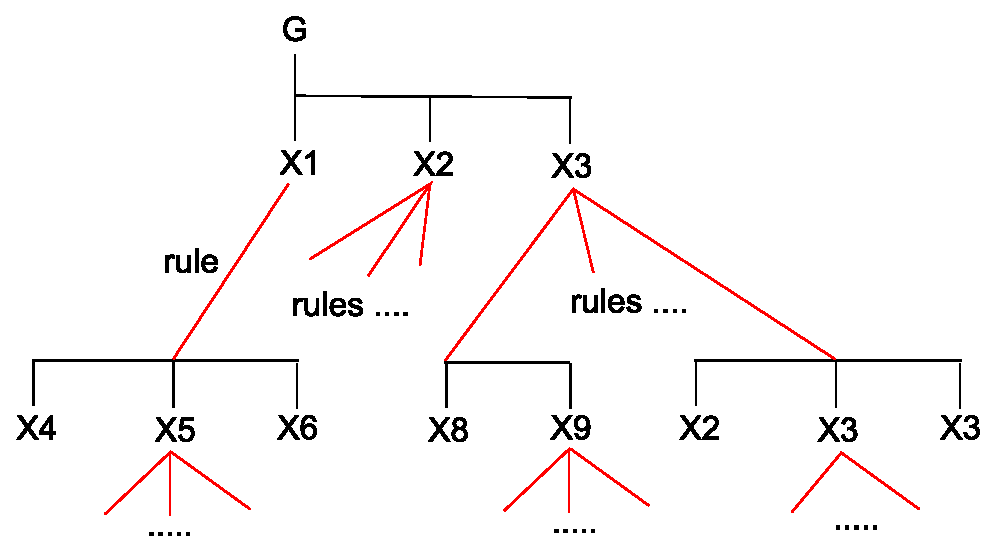
\includegraphics[scale=0.8]{and-or-graph.eps}
% \caption{Plots of mean and variance; output vs input}
\end{figure}

\textbf{Complexity.}  If $m$ is the average number of rules applicable to a head predicate, $n$ is the average number of arguments for each rule, and $h$ is the depth of the search tree, then the size of the tree is $O((m \cdot n)^h)$.  Let me make a wild guess that $m \approx 30, n \approx 5, h \approx 5$, then size $\approx 10^{11}$.  This sounds manageable, but don't forget that the complexity of learning is the exponentiation of this!  So it is important to keep things simple at this stage.

\textbf{Efficient deduction.}\\
1.  Inference is often grounded by facts in \textbf{Working Memory} (ie, things that the AGI is currently paying attention to), though it may also be grounded by facts recalled from LTM (Long Term Memory).  Perhaps an efficient search algorithm should \textit{simultaneously} use backward chaining from the goal and forward chaining from ground facts under current attention.\\
2.  Given a head predicate, the KB server can quickly retrieve a list of all rules with that predicate by looking up an index.  Also, this list can be assumed to be sorted in order of confidence (remember that each rule is associated with a frequentist confidence).  This order may provide a basis for best-first / heuristic search\\
2.  Maybe the search should be randomized, and maybe it can start from the ``middle'' (ie, we generate an initial proof that is incorrect or incomplete, then repeatedly mutate it to make it correct)\footnote{This idea is inspired by the GSAT and WalkSAT algorithms for propositional logic.}.  This suggests using an evolutionary algorithm, but EA's may be slow. \{ TO-DO:  explore this idea further \}

Solving this search problem is very important because inductive learning also depends on such a search.

\subsection{Loopy inference}

\section{Abduction}
\label{sec:abduction}

(Logic-based) abduction and induction are closely related;  they are 2 faces of the same coin.  In both cases we seek a hypothesis $H$ that together with background knowledge $B$, entails a positive example $e^+$:
$$ B \cup H \vdash e^+ $$
the only difference is that for abduction, $H$ is ground (ie, contains no variables); and for induction, $H$ is non-ground.

In classical logic, the algorithm for abduction is identical to deduction (backward chaining) except that the termination criterion is different.  In deduction the leaves of the search tree should be ground facts in the KB (which are believed to be true).  For abduction, the leaves should be so-called \textbf{abducibles}, which are propositions that can be assumed to be true.  For example, ``rain'' is a common occurrence and thus can be assumed to be true in order to account for the grass being wet.

Under probabilistic logic, we no longer need the notion of abducibles.  Interestingly, in this case the algorithm for abduction becomes almost identical to that of deduction, with the exception that deduction starts with an unknown fact whose truth is to be determined; whereas abduction starts with a known fact in need of explanations.  The 2 search spaces are exactly the same.

TO-DO:  unfinished.

%Z abduction sometimes gives out-of-bounds Z values.\\
%\hspace*{1cm} $ z_1 \widetilde \vee z_2 = high $\\
%\hspace*{1cm} $ z_1 = low $\\
%\hspace*{1cm} $ \Rightarrow z_2 > 1.0 $
%
%Also, there are always 2 solutions, and they are within-bounds in the $z_1 > 0.5$ regime. Why?
%
%In fact, abduction using a rule with a point-Z-value is very unnatural.  Perhaps if we use $P(Z)$ the problem will be resolved?  But the ``2 roots'' problem seems to remain...

\chapter{Pattern recognition}
\minitoc

\section{The theory-based theory}

Concept formation (or ``categorization'' in the cognitive science literature, \citep*{Murphy2002}, \citep*{Cohen2005}, \citep*{Margolis1999}, \citep*{Lakoff1987}) is the task of using machine learning to learn common-sense concepts (\citep*{Nakamura1993}, \citep*{Wrobel1994}).  \citep*{Wrobel1994} has summarized the following properties of human concepts:
\begin{compactenum}[1.]
\item concepts often have non-necessary features
\item disjunctive concepts (there may not be any features that are shared by all members of a concept)
\item relational information (seems to require first-order logic to represent)
\item some features are themselves concepts
\item typicality (people can often rank examples according to typicality, eg the most typical fruit is orange)
\item basic levels (people are more adapt at categorization at certain basic levels, eg naming an object ``chair'' rather than ``office chair'' or ``a piece of furniture'')
\item superordinate distance (eg ``chicken'' is rated more similar to ``animal'' than to ``bird'')
\item unclear cases (eg ``is tomato a fruit?'')
\item context-dependent effects
\item goal-dependent effects
\end{compactenum}

There are two major theories of categorization:  In the \textbf{Classical view} a concept is defined by a set of defining features which are individually necessary and sufficient.  This view has very few adherents now.  The other major theory is the \textbf{Exemplar view}, which classifies instances based on their similarity (eg a distance metric) to a set of existing exemplars.

In my opinion, also shared by \citep*{Murphy1985} and \citep*{Wrobel1994}, the most satisfactory solution (aka the \textbf{theory-based theory}) is to view categorization as an \textit{inference} process, where concept formation means constructing \textit{explanations} of why certain objects belong to a concept.

\chapter{Belief revision}
\label{ch:belief-revision}
\minitoc

Belief revision concerns the problem of conflicting conclusions and, in the extreme, contradictions.

One simple question is:  If we arrive at two P(Z) distributions from two separate inference chains, how to combine the answers?

It seems that this is related to statistical inference.  Suppose we have a population.  A set of observations gives the estimate of the mean and variance:\\
\hspace*{1cm} $x_1, x_2, ..., x_{n_1} \sim Beta(\mu_1, v_1)$\\
Another set of observations gives another pair of estimates:\\
\hspace*{1cm} $y_1, y_2, ..., y_{n_2} \sim Beta(\mu_2, v_2)$\\
The question is to find a reasonable way to combine the 2 sets of observations to give a new estimate:\\
\hspace*{1cm} $x_1, x_2, ..., y_1, y_2, ... \sim Beta(\mu_0, v_0)$\\
In other words, how to express $(\mu_0, v_0)$ in terms of $(\mu_1, v_1)$ and $(\mu_2, v_2)$?

Maybe the $\mu_0$ is just the weighted average of $\mu_1$ and $\mu_2$?  $n_1, n_2$ can be assumed to be equal to the supports $w_1, w_2$ which can be calculated from the confidences $c_1, c_2$.

Some assumptions in the above may not be entirely justified:  the population size is typically small and the 2 samples may have overlap, ie, not independent.

\section{Justifications}

\section{Common assumptions vs deliberate assumptions}

\section{Theory revision}

See \S\ref{sec:ILP}.

\chapter{Meta-reasoning}
\label{ch:meta-reasoning}
\begin{flushright}
\emph{I think I think, therefore I think I am.}
\end{flushright}
\minitoc

The term ``meta-reasoning'' may refer to 2 things:\\
1. The ability to \textbf{reason about reasoning}, which is what this chapter is concerned with;\\
2. Scheduling reasoning tasks to achieve best results with limited computational resources (I have not thought about this problem yet).

An excellent survey of meta-reasoning in the \#1 sense is \citep*{Constantini2002}.

In the Tell-Learn loop, we see that we need a special predicate credible() to increase the probability of a statement via a side-effect.  But that may not be the only meta-reasoning move we can make.

Another example is the $B \leftrightarrow Z$ conversion of ``traitor'' and ``patriot'' (\S\ref{sec:PZ-meta-reasoning}).

\section{Higher order logic}

\chapter{Learning}
\label{ch:machine-learning}
\begin{flushright}
\emph{Rewards and punishment is the lowest form of education.} --- Zhuangzi (4th Century BC)
\end{flushright}
\minitoc

\section{``Learn by talking''}
\label{sec:learn-by-talking}

This is probably the most efficient learning method.  (As Martin Magnusson pointed to me, \citep*{Perlis1996} explored the possibility where a human is able to teach an AI via natural-language conversations.  The paper contains hypothetical examples of some such conversations.)

\textbf{The Tell-Learn loop.}  Translate a natural language sentence into a logical formula.  Then the logical formula will directly enter the KB as knowledge, which is a very efficient way of learning.

The main difficulties in this loop are:
\begin{compactenum}[1.]
\item  The assimilation of the fact into the KB, which requires belief revision
\item  The translation from natural language to logic;  sometimes this require abductive reasoning even when the NL parser does an adequate job
\item  Surprisingly, inductive learning is also needed (see \S\ref{sec:ILP})\\
\end{compactenum}

The base logic should be:\\
1. simple, for machine learning\\
2. close to NL, for easy translation from NL to logic.

\section{Inductive logic learning}
\label{sec:ILP}

Inductive learning using logic is studied under the heading ILP (inductive logic programming; an excellent and up-to-date survey of which is \citep*{Konstantopoulos2008}).  The area known as theory revision is also essential to AGI (an excellent new book on ILP that discusses theory revision is \citep*{DeRaedt2008}).  \{ cite older books on ILP \}.

\textbf{Why is ILP needed?}  From my observations, when people use natural language to express ideas, they usually leave many \textbf{gaps} that must be filled by abductive or inductive reasoning.  A parser can translate NL sentences into logic \textit{literally}, but the resulting KB would be incapable of reasoning.

Filling in the logical gaps is very hard for humans because the inference of the gaps are inaccessible to conscious thinking.  Therefore, an inductive machine learner is required to perform this function.

\subsection{Complexity of ILP}

THe main task of ILP is to search in the hypothesis space $\mathbb{H} \;$ specified partly by the logical syntax (such as P(Z) logic) and partly by background knowledge (eg what kind of predicates are present).  The hypothesis space is structured into a lattice with a partial order (usually denoted $ \preceq $).  The partial order can be one of \textbf{$\theta$-subsumption}, LGG (\textbf{least general generalization}), or \textbf{logical entailment}.  These have subtle differences, with logical entailment being the most rigorous.  The searcher can traverse up and down the lattice, corresponding to \textbf{generalization} and \textbf{specialization} of the hypothesis.  These 2 are known as \textbf{refinement operators}.  Because there are so many ways to generate hypotheses in FOL (with many predicates to choose from, and the possibility of introducing variables as desired), the branching factor is extraordinarily high.  Also, the lattice can be infinite, so we need to limit its depth.

Another problem is that, once a hypothesis has been generated, it must be tested against the rest of the KB for \textbf{consistency}.  The consistency check must also be limited in depth, but even then it is very time-consuming.

Much of the complexity of induction occurs in the ``inventive step'', whereby a new rule is generated.  The inventive step can draw upon knowledge from the entire KB, which makes it combinatorially explosive.  Currently the most promising idea I have is to ``recall similar examples'' -- that means, we perform an \textbf{associative memory search} to recall examples similar to the current experience, and only then do we try to generalize from the experience plus the recalled examples.  But this strategy merely pushed the responsibility to the associative memory to recall only the most \textbf{salient / relevant / interesting} examples.  Still, this trick seems to be more efficient than blind search.

Another promising idea is that some of the more intensive processing can be performed during \textbf{sleep}.

\subsection{Complexity of theory revision}

Let $\mathbb{H} \;$  denote the hypothesis space (ie, space of all logic formulae).  The size of $\mathbb{H} \;$ is huge (see above).\\
A logical theory $T$ is a set of hypotheses, $ \{ h_i | h_i \in \mathbb{H} \; \} $.  Note that $ T \in 2^{\mathbb{H}} \;$ which is a hugely huge space.\\
Let $E$ denote the set of examples $\{ e_1, ... \}$ that should be covered by the target theory.\\
So we're seeking an optimal theory $T^*$ such that it covers all examples and is succinct, ie:\\
\hspace*{1cm} $ T^* \vdash E $ \quad and \quad $ |T^*| $ is minimal.

There is hope, since we can \textit{seed} the initial theory with human knowledge.  In other words, we can start with $T_0$ which contains a large number of logic statements translated from NL.

Even if we do that, we can realistically only store one theory in memory.  When we evaluate a new hypothesis $h$ to cover an example $e$, ie, to test whether\\
\hspace*{1cm} $h \cup T \vdash ? \; e $\\
we have to bear in mind that we are just testing the hypothesis $h$ w.r.t. \textit{one} background theory.  This means that $h$ may have a different score when $T$ changes;  but unfortunately we cannot realistically keep track of different scores of $h$ against different theories.  In other words, the scores we keep will be somewhat \textit{inaccurate} and are \textit{relative} to a constantly changing candidate theory.

%\section{Evolutionary algorithms}
%
%It seems that EA, as a global optimization technique, can be a good choice for the ILP search.  There are two general approaches to GA (\citep*{Freitas2002}):
%
%In the \textbf{Pittsburgh approach}, each individual in the EA population represents \textit{a set of rules}, ie, an entire candidate solution.
%
%In the \textbf{Michigan approach}, which departs from conventional EA's, each individual represents \textit{a single rule}, ie, a part of a candidate solution.
%
%It seems to me that we need the Michigan approach.
%
%TO-DO:  how to learn hybrid logical rules.
%Learning of Z rules is based on examples with explicit Z values;\\
%Learning of P rules is based on examples that are true or false.\\
%So they may be learned independently?
%
%Besides Michigan vs Pittsburgh, one more thing is the role of a lot of background knowledge.  How might this change things?

\subsection{Algorithm}

I look at the problem from a perspective that is slightly different from the one prevalent in the ILP literature.  Most ILP methods search in the \textit{hypothesis space}, but I find it easier to think about the problem in \textit{proof space}:\\

\begin{compactenum}[\textbullet ]
\item  My algorithm searches for explanations of \textit{one incoming fact} while inventing (possibly many) hypotheses along the way.
\item  The hypothesis-space algorithm, on the other hand, focuses on \textit{one hypothesis}.  It would pick some examples (past or incoming facts) and move around the hypothesis lattice in order to cover them, ie, keeping a score of the numbers of positive and negative examples that are covered or not.  And it seeks the hypothesis with the best score.\\
\end{compactenum}

The main problem with hypothesis-space search is that all the examples relevant to a hypothesis do not come at the same time.  In real experience, the examples are usually scattered over a long time span.

%\{ TO-DO: how to combine the 2? \}

\section{Reinforcement learning} \index{reinforcement learning}

The goal of RL is to learn an optimal policy which is a function $\pi: \{states\} \rightarrow \{actions\}$.

RL can learn to:\\
1.  conversate with humans (eg in chat rooms)\\
2.  write programs\\
3.  crawl the web to learn things\\
and do all these without the need for human programming, so it is cost-effective.

\subsection{Relational reinforcement learning}

\chapter{Natural language}
\begin{flushright}
\emph{The fish trap exists because of the fish; once you've gotten the fish, you can forget the trap. The rabbit snare exists because of the rabbit; once you've gotten the rabbit, you can forget the snare. Language exists because of meaning; once you've gotten the meaning, you can forget language.}\\ --- Zhuangzi (4th Century BC)
\end{flushright}
\minitoc

\section{Natural language is not essential to AGI}

Needless to say, fully solving the natural language problem is AGI-complete.  This however is not a show-stopper.  Our ultimate goal is to reach the \textbf{RSI point} (\S\ref{sec:RSI}) with as little effort as possible.  Which means we only need the most basic system that can automatically write programs for us.  Such a system only needs to accept commands in a \textit{restricted} subset of English.  Thus, for all our purposes an NL module that can parse restricted English would suffice.

\section{Unification-based grammars}

The family of unification-based grammars includes LFG (Lexical Functional Grammar), HPSG (Head-Driven Phrase Structure Grammar), and PATR grammar.  The unification algorithm used in unification-based grammar is the same as the unification algorithm used in logic.  This is further evidence that the brain employs first-order symbolic processing.

\section{Cognitive linguistics}

Currently we are using the ``formal semantics'' approach.

\{ TO-DO:  How may cognitive linguistics affect the design of the natural language subsystem? \}

\section{Abduction as interpretation}
\label{sec:AbductionAsInterpretation}

\subsection{A detailed example}

The general sequence is:\\
\hspace*{1cm} tokenization $\rightarrow$ POS-tagging $\rightarrow$ syntax parsing $\rightarrow$ semantic parsing\\
which should be familiar to everyone with experience in NL processing.

I will explain the details using a simple example:\\
\hspace*{1cm} ``I love Mary''

The crucial thing is that we represent everything in a logic-based framework. First we represent the sentence as "raw data" (ignoring tenses to simplify matters):\\
\hspace*{1cm} $\mbox{sentence}(e_0)$\\
\hspace*{1cm} $\mbox{lexeme-I}(e_1)$\\
\hspace*{1cm} $\mbox{lexeme-love}(e_2)$\\
\hspace*{1cm} $\mbox{lexeme-Mary}(e_3)$\\
\hspace*{1cm} $\mbox{begins-with}(e_0, e_1)$\\
\hspace*{1cm} $\mbox{follows}(e_2, e_1)$\\
\hspace*{1cm} $\mbox{follows}(e_3, e_2)$\\
where:\\
\hspace*{1cm} the $e_i$'s are \textbf{entities} (logical constants).\\
\hspace*{1cm} the entities $e_1$, $e_2$, and $e_3$ are words.\\
\hspace*{1cm} follows() means a word follows another word in a sentence.

Up to now, all we have is a sentence as raw text (without meanings).  The next step is to recognize parts of speech (nouns, verbs, adjectives, etc). We can use logical rules to do this.

An example logical rule is:\\
\hspace*{1cm} $\mbox{lexeme-Mary}(X) \rightarrow \exists e \; \mbox{parse-as}(e, X) \wedge \mbox{noun}(e)$\\
which simply means that the word "Mary" is a noun. X is a variable (implicitly universally quantified). $e$ is a new entity, which instantiates to $e_4$ when the rule is applied.

We can also use logical rules to parse syntax. We can perform ``VP $\leftarrow verb + noun$'' with this rule\footnote{We need this special rule:\\
\hspace*{1cm} $\mbox{follows}(X_1, X_2) \wedge \mbox{parse-as}(X_1, X_3) \wedge \mbox{parse-as}(X_2, X_4) \rightarrow \mbox{follows2}(X_3, X_4)$ }:\\
\hspace*{1cm} $\mbox{verb}(X_1) \wedge \mbox{noun}(X_2) \wedge \mbox{follows2}(X_2, X_1) \rightarrow \exists e \; \mbox{parse-as}(e, X_1, X_2) \wedge vp(e)$\\
which creates a new entity $e_5$ which is a VP.

Assume that eventually we have a parse of the sentence S, $e_6$. Notice that up to now, it's all syntax parsing.

Next we perform semantic parsing.  The key is to generate partial meanings for phrases, such as the verb phrase ``loves Mary''.

\textbf{Lambda operator.}  In formal semantics, it is customary to use the $\lambda$ operator to represent the meaning of phrases.  The reason is that first-order logic do not have the expressive power to represent such phrases.  For example, the VP ``loves Mary'' denotes ``somebody's loving Mary'', which may be represented as $love(\_ \,,mary)$; but that is not a well-formed formula in FOL.  Instead we can represent it using the $\lambda$ expression $\lambda x \; love(x,mary)$.  This is no longer FOL, but is a so-called \textit{quasi-logical} form.  I propose to use an alternative method which is within FOL.  It employs the composition functor.

\textbf{Composition functor.}  (See also \S\ref{sec:CompositionFunctor})  Under this method, all phrases are represented by compositions.  For example, the VP ``loves Mary'' can be represented by $comp(loves,mary)$, or in short-hand $loves * mary$.  This composite is a \textit{first-order object}, which cannot be further reduced, but when we compose it with $john$, we get $john * (loves * mary)$ which is equivalent to the first-order statement $loves(john,mary)$.  So we need special inference rules to convert such composites into statements.

I think this method is superior to $\lambda$ because the meanings of phrases can be represented by first-order objects.  It also makes semantic parsing very intuitive.

\{ TO-DO:  Explain semantic parsing with examples. \}

%A semantic rule is similar to a syntactic one:\\
%\hspace*{1cm} $\mbox{lexeme-love}(X) \rightarrow \exists e \; \mbox{parse-as}(e, X) \wedge \mbox{verb}(e) \wedge \mbox{means}(e, \mbox{concept-love})$\\
%
%\hspace*{1cm} $\mbox{verb}(X_1) \wedge \mbox{np}(X_2) \wedge \mbox{follows2}(X_2, X_1) \wedge \mbox{means}(X_1, Y_1) \wedge \mbox{means}(X_2, Y_2)$\\
%\hspace*{1cm} $\rightarrow \exists e \; \mbox{parse-as}(e, X_1, X_2) \wedge vp(e) \wedge \mbox{means}(e, comp(Y_1,Y_2))$\\
%
%For example, we can augment the syntactic rule\\
%\hspace*{1cm} $\mbox{VP} \leftarrow \mbox{verb}, \mbox{NP} $\\
%with\\
%\hspace*{1cm} $\mbox{VP}(\mbox{comp}(Sem_1,Sem_2)) \leftarrow \mbox{verb}(Sem_1), \mbox{NP}(Sem_2)$\\
%where the $Sem$'s are variables containing the ``semantics'' of phrases.\\
%\hspace*{1cm} $\mbox{S} \leftarrow \mbox{NP}, \mbox{VP} $\\
%\hspace*{1cm} $\mbox{S}(Predicate) \leftarrow \mbox{NP}(Subject), \mbox{VP}(Subject * Predicate) $\\
%\hspace*{1cm} $\mbox{VP}(X) \rightarrow \mbox{com}(\mbox{loves},\mbox{mary})$\\
%which creates a new entity $e_7$ with the meaning of "love".\\
%\hspace*{1cm} $\mbox{lexeme-love}(X_1) \rightarrow \exists e \; \mbox{concept}(e) \wedge \mbox{means}(e, \mbox{concept-love})$\\
%
%The final step of semantic parsing uses a special trick,  ``de-reification'' (\S\ref{sec:reification}):\\
%\hspace*{1cm} (assume that $e_{8}, e_{9}$ denote the persons John and Mary)\\
%\hspace*{1cm} $\mbox{de-reify}(\mbox{concept-love}, e_{8}, e_{9})$\\
%which generates the logical statement:\\
%\hspace*{1cm} $\mbox{loves}_1(e_{8},e_{9})$\\
%
%Finally we have:\\
%\hspace*{1cm} $\mbox{means}(e_0, \mbox{loves}_1)$

\section{Universal logical form}
\label{sec:UniversalLogicalForm}

An immediate question is how to translate ``nearly every text sentence under the sun'' into logical form.  To which we employ several rules to quickly reduce the problem space:

1.  Every noun (except special nouns such as pronouns) corresponds to a concept which is represented by a predicate.  For example, the word:chair corresponds to the concept:chair and is represented by the predicate \texttt{concept-chair()}.

%2.  Every verb

%3. 

\section{Some example English sentences}
\label{sec:English-examples}

\chapter{Memory systems}
\begin{flushright}
\emph{Computer science has only three ideas: cache, hash, trash}\\ --- Greg Ganger, CMU
\end{flushright}
\minitoc

\section{Associative memory}
\label{sec:associative-memory}

Associative recall can greatly facilitate inductive learning.

Sometimes fuzzy associations may be desirable.

The KB being in first-order logic poses problems for fuzzy associations.  It is unlike associative neural networks which may be closer to propositional logic.

\section{Efficient rule selection}
\label{sec:EfficientRuleSelection}

\{ TO-DO:  This idea is problematic.  It only works if the approximate oracle is correct a high percentage of the times;  but this is highly suspect.  \}

Given:\\
1. The goal (ie, the conclusion of the proof)\\
2. The premises (ie, facts residing in Working Memory)\\
Try to predict:\\
3. The rules involved in the proof

Each data point would be:\\
1.  goal (a grounded fact)\\
2.  premises (set of grounded facts)\\
3.  a critical rule

So it seems:\\
\{ fact \} $\times$ \{ set of facts \} $\rightarrow$ rule

Using multidimensional scaling, we can map a fact to its coordinates in a high-dimensional space.

Then we can partition the high-dimensional space into grids, and to each grid assign a bucket of rules.  We need some way to partition the high-dimensional space.  But we can also partition the space of data points into many categories?

\chapter{Planning and acting}
\label{ch:planning-acting}
\minitoc

\section{``Procedural subsumes Declarative''}
\label{sec:proc-subsumes-decl}

So far, we have only talked about the \textbf{declarative} aspect of AGI.  Now we need to consider the \textbf{procedural} aspect.

It seems natural that the procedural system should subsume the declarative system:
\begin{figure}[H]
\centering
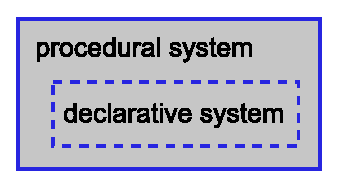
\includegraphics{Procedural-subsumes-Declarative-system.eps}
\end{figure}
\vspace{-0.5cm}

The procedural system communicates with the declarative system via various types of \textbf{querying}.  The declarative system itself has no means of performing actions;  its only function is question-answering.  There may be exceptions, but the general rule can be captured by the slogan \textit{``Procedural subsumes Declarative''}.

\section{The action language}
\label{sec:ActionLanguage}

We have represented declarative knowledge using a logical language; now we should represent procedural knowledge with a similar action language.

The following are examples of ``actions'':\\
1. say "hello"\\
2. open a file\\
3. print 1...100\\
4. repeat printing N until the user presses the Esc key

Do they sound like programming language tasks?  Thinking along this line, it seems advantageous that \textit{the action language should be a conventional programming language} such as C++, Java, Lisp,  Prolog, etc.

So the procedural system expresses actions in a programming language.  Those actions can be executed via the compiler or interpreter of that language.  In some situations, it is more convenient if the language can be interpreted.

The action output of the Procedural System can be of 3 forms:\\
1. a statement that is immediately interpreted and executed\\
2. a program that needs to be compiled\\
3. a program fragment that becomes part of the Procedural System

\#3 is actually a form of procedural learning.

\section{Procedural learning}
\label{sec:ProceduralLearning}

When the procedural language is complex, learning may be more difficult.  So there may be a need to restrict the procedural language.  %Secondly, there may be a need to put the learned procedures within a meta-controller framework so as to control them better.

Learned procedures can be inserted into the Procedural System at certain hook points.  Each hook point represents a context, for example ``We get here when the user presses the Esc key''.  The procedural learning algorithm should take such contexts into consideration.

``Learn by talking'' is also applicable to procedural learning.

\section{Deductive planning}
\label{sec:deductive-planning}

A classical planning problem is represented by states and operators (actions).  Each operator has its precondition and effect.

In deductive planning based on situation calculus, actions are represented as terms, with the special predicates \texttt{do()} and \texttt{poss()}.

An advantage of deductive planning is that the Procedural System only needs to be a inference engine and nothing else.

One difficulty here is how to represent states, actions, preconditions, and effects;  especially actions.  I can put the cup on the table.  The current state is represented implicitly by all the facts in KB.  The actions are a special class of facts related to possibilities.  ``Water conducts electricity'' is a fact;  But ``water can conduct electricity'' is a possible action?  

Also, DP has a problem in that it only pursues one goal at a time.

\subsection{Combining reinforcement learning and deductive planning}

Both RL and DP may generate actions, and so they can be in conflict.

DP says:  ``If I do X, Y may happen as a result''.\\
RL says:  ``At state S, if I do X, the reward may be high''.

It seems that RL can be entirely absorbed into the DP paradigm.

\chapter{Program synthesis}
\minitoc

The most critical milestone of our project is to create a system that can perform simple automated programming.  Traditional program synthesis systems are hard to use because:\\
1. They require \textit{formal specifications} of program requirements, which are often as hard to write as the programs themselves, sometimes even harder.\\
2. The proof search is \textit{too slow} for any problem of practical size, or the systems often require human interaction for guidance.\\

My proposal to solve these two problems are, respectively:\\
1. Allow \textbf{informal} specification of programming goals.  This means using (restricted) natural language, including vague / probabilistic language.\\
2. In order to speed up the program search, it seems that the only viable solution is to use knowledge to guide the search.  This is something that has been recognized in the AI community for a long time --- no clever search algorithm or heuristic can improve the search significantly, without domain-specific background knowledge.  Machine learning can be used to acquire such knowledge, but it is often an extremely difficult problem in itself; and we are also talking about a large body of background knowledge.  As I have argued in \S\ref{ch:machine-learning}, the most efficient way to acquire knowledge is to give up machine learning and simply \textbf{learn by talking}.

As with many AI problems, the program synthesis problem can be construed as a search, and we have the usual choice of top-down and bottom-up. % I think the more promising approach is top-down but is this really true?

\section{Formal program synthesis}

\chapter{Value judgments}
\begin{flushright}
\emph{The real question is not whether machines think but whether men do.}\\
--- B F Skinner
\end{flushright}
\minitoc

\section{My stance on AGI friendliness}

I do not have a rigorous theory for AGI friendliness and I'd be very suspicious of any such theory.  But I believe that AGI technology should be made widely available to the general public, because the distribution of power is the best safeguard against abuses of AGI.

Other than that, the AGI should be subject to certain laws that prevent exploitation (eg, unlimited growth or taking up of physical resources).  That would be the job of governments.

\section{Sentient vs non-sentient AGI}


\chapter{Vision and other senses}
\label{ch:vision}
\minitoc

TO-DO:  transfer web pages to here.

\section{Logic-based vision}

% \chapter{Business aspects}
\begin{flushright}
\emph{Sure now what's worth doing, is worth doing for money.}\\
--- Wall Street (1987 movie)
\end{flushright}
\minitoc

\section{Capitalism, AI, and the Singularity}

Of course, it is impossible to predict things past the Singularity, but my view of the Singularity is more conservative in the sense that I believe human life will remain unchanged in some essential aspects.  My premise is that capitalism will persist after the advent of AI.

\section{My political stance}

As an AGI entrepreneur, I need not be involved in politics, and I have no intention to do so, but some people are frequently trying to politicize the issue to gain an advantage over me, so I am forced to clarify a few things here.

Firstly, I am not anti-American.  My goal is to create a global AGI project without bias towards a particular nationality.  This does not mean that I am advocating to put an end to nationalism.  The internet allows us to work across geographic boundaries, so the conditions are right for this kind of trans-national collaboration.

Secondly, I think open source as a software business model is flawed.  Companies need to protect new ideas to give people incentives to innovate.

\underconst

\section{Collaborative platform}

From 2010 April onwards, all \href{http://spreadsheets.google.com/ccc?key=0Ah3_S9SExak-dFA5YTQ2anRfOWxrR2JMM0toekpvVEE&hl=en}
{accounting information} of this project are disclosed.

\subsection{Virtual credits}

\textbf{BitCoin.}

\subsection{Voting scheme}


\chapter*{Acknowledgments}

In addition to the people listed on the title page, I'd like to thank the AGI mailing-list participants for years of discussions.

%\glossary{name={},description={}}
\glossary{name={ATP},description={automated theorem proving}}
\glossary{name={BDI},description={belief-desire-intention (architecture)}}
\glossary{name={CDF},description={cumulative distribution function}}
\glossary{name={CNF},description={conjunctive normal form}}
\glossary{name={DNF},description={disjunctive normal form}}
\glossary{name={DP},description={deductive planning}}
\glossary{name={EA},description={evolutionary algorithm}}
\glossary{name={FOL},description={first-order logic}}
\glossary{name={HOL},description={higher-order logic}}
\glossary{name={ILP},description={inductive logic programming}}
\glossary{name={KB},description={knowledge base}}
\glossary{name={KR},description={knowledge representation}}
\glossary{name={LBAI},description={logic-based AI}}
\glossary{name={LGG},description={least general generalization}}
\glossary{name={LTM},description={Long-Term Memory}}
\glossary{name={MDL},description={minimum description length}}
\glossary{name={NL},description={natural language}}
\glossary{name={NP},description={noun phrase}}
\glossary{name={NR},description={natural reasoning (= common-sense / human-like reasoning)}}
\glossary{name={PCA},description={principal component analysis}}
\glossary{name={PDF},description={probability density function}}
\glossary{name={RL},description={reinforcement learning}}
\glossary{name={RSI},description={recursive self-improvement}}
\glossary{name={SAT},description={logical satisfiability}}
\glossary{name={SLD},description={selective linear definite clause resolution}}
\glossary{name={SLS},description={stochastic local search}}
\glossary{name={SVM},description={support vector machines}}
\glossary{name={TV},description={truth value}}
\glossary{name={VP},description={verb phrase}}
\glossary{name={WM},description={Working Memory}}
\glossary{name={ZOL},description={zeroth-order logic (= propositional logic)}}

\printglossary
\addcontentsline{toc}{chapter}{Glossary}

\bibliographystyle{plainnat}
\bibliography{JJJJ}

%\printindex
%\addcontentsline{toc}{chapter}{Index}

\end{document}
